\documentclass[12pt,oneside,a4paper]{article}
\usepackage[backend=biber,style=numeric]{biblatex}
\usepackage[table]{xcolor}
\usepackage{todonotes}
\usepackage{caption}
\usepackage{hyperref}
\usepackage{graphicx}
\usepackage{float}
\usepackage{changepage}
\usepackage{booktabs}
\usepackage{tabularx}
\newcolumntype{Y}{>{\arraybackslash\hspace{0pt}}X}
\usepackage[left=2.5cm, right=2.5cm, top=2.5cm, bottom=2.5cm]{geometry}
\pagestyle{plain}
\usepackage{url}
\usepackage{fancyhdr}
\pagestyle{fancy}
\renewcommand{\headrulewidth}{2pt}
\renewcommand{\footrulewidth}{1pt}
\usepackage{adjustbox}
\usepackage{lipsum}
\usepackage{mwe}
\usepackage{listings}


\begin{document}

%Title Page
\begin{titlepage}
    \centering
    {\scshape\large AY 2023/2024 \par}
    \vfill
    
\includegraphics[width=0.5\textwidth]{Images/poli.jpg}\par\vspace{1cm}
    %{\scshape\LARGE Politecnico di Milano \par}
    \vspace{1.5cm}
    {\huge\bfseries DD\@: Design Document \par}
    \vspace{2cm}
    {\Large {Filippo Gentili\quad Emanuele Greco\quad Marco Giulio Grilli}\par}
    \vfill
    {\large Professor\par
        Matteo \textsc{Rossi}}
    \vfill
    {\large \textbf{Version 1.0}\\ \today \par}
\end{titlepage}

%Table of Contents
\tableofcontents

\pagebreak

%Begin of documents
\section{Introduction}

\subsection{Purpose}
This document aims to offer a comprehensive and detailed elucidation of the forthcoming system to be. The primary focus lies on elucidating the chosen architecture, delineating the various modules constituting the system, and illuminating the interfaces that facilitate their interconnection. In addition, a runtime perspective is presented, which is complemented by interaction diagrams, providing a visual representation of the message exchange dynamics among the different components. Lastly, attention is directed towards aspects such as implementation strategies, testing methodologies, and the integration processes that will be undertaken. These components collectively contribute to a thorough understanding of the system, encompassing its design, operational aspects, and the sequential phases leading to its realization.


\subsection{Scope}
The platform provides different actors that will use it, such as Users, Educators and Students.
\begin{itemize}
    \item \textbf{Users} can access the platform in order to register themselves up, as either a Student or an Educator, and to check other users' profiles.
    \item \textbf{Educators} can create tournaments and battles as well as manage both of them, they can also create badges and evaluate projects presented by students teams. Moreover, they can define specific rules, through a determined language, and variables used to create constraints for the badges. 
    \item \textbf{Students} can participate in battles and tournaments by enrolling themselves in, can form teams with their friends or join one and can see their personal rank and score for a specific tournament.
\end{itemize}


\subsection{Definitions, Acronyms, Abbreviations}

\subsubsection{Definitions}
\begin{itemize}
    \item \textbf{Rule}: It is a mathematical confrontation between variables to define a badge.
    \item \textbf{Variable}: A specific type of data stored in the database, used for the creation of rules.
\end{itemize}

\subsubsection{Acronyms}
\begin{itemize}
    \item \textbf{RASD}: Requirements Analysis and Specification Document
    \item \textbf{S2B}: System To Be
    \item \textbf{DD}: Design Document
    \item \textbf{UI}: User Interface
    \item \textbf{UX}: User Experience
    \item \textbf{DBMS}: DataBase Management System
\end{itemize}


\subsubsection{Abbreviations}
\begin{itemize}
    \item \textbf{Gn}: Goal number n
    \item \textbf{Rn}: Requirement number n
    \item \textbf{ID}: Identification Number
\end{itemize}


\subsection{Revision History}
\begin{itemize}
    \item \textbf{Version 1.0}: First release.
\end{itemize}

\subsection{Reference Documents}
In this Design Document we have used the following referenced documents:

\begin{itemize}
    \item Requirements Analysis and Specification Document
    \item Assignment RDD AY 2023-2024
    \item Course Slides from Software Engineering 2
\end{itemize}


\subsection{Document Structure}
\begin{itemize}
    \item \textbf{Section 1: Introduction}\\ This section provides a succinct overview of the forthcoming document, offering essential details such as definitions, acronyms, and abbreviations that will be encountered throughout its contents. It serves as a helpful introduction, ensuring readers are equipped with the necessary background information to navigate and comprehend the document effectively.
    \item \textbf{Section 2: Architectural Design}\\ This section is specifically directed towards the developer team, aiming to provide an in-depth exploration of the system's architecture. The initial segment delves into the chosen paradigm and outlines the overall segmentation of the system into distinct layers. Additionally, it furnishes a high-level depiction of the system, accompanied by an introduction to the modules constituting its nodes. Concluding this section is a detailed exposition of the tiers that collectively constitute the S2B, providing a concrete and comprehensive understanding of its structural components.
    \item \textbf{Section 3: User Interface Design}\\ This section is a valuable resource tailored for the graphical designers involved in shaping S2B. It includes a succinct collection of mockups showcasing the application's visual representation, while most of the mockups have been included in the RASD, which is heavily linked with this document. These mockups specifically depict the user interface and overall client-side experience. Designers can leverage this section to gain a clear understanding of the intended aesthetics and user journey within the system.
    \item \textbf{Section 4: Requirements Traceability}\\ This section serves as a pivotal connection between the RASD and the DD document. It establishes a comprehensive mapping that links the requirements and goals articulated in the RASD with the logical modules presented in this document.
    \item \textbf{Section 5: Implementation, Integration and Test Plan}\\ The final section is tailored once more for the developer team, elucidating the systematic procedures governing the implementation, testing, and integration of the components within our S2B. It provides an exhaustive account of the core functionalities inherent in the system, accompanied by a thorough report detailing the methodologies for their implementation and the corresponding testing protocols. This section serves as a comprehensive guide for developers, offering insights into the operational aspects and quality assurance measures associated with the S2B's constituent components.
\end{itemize}

\clearpage

\section{Architectural Design}

\subsection{Overview}
This section provides a comprehensive overview of the architectural elements that constitute the system, delineating their interactions and detailing the chosen replication mechanism aimed at rendering the system distributed. The content delves into the fundamental components that make up the system's architecture, elucidates how these elements interact with each other, and underscores the specific replication mechanism selected to imbue the system with a distributed nature. This information collectively contributes to a deeper understanding of the structural framework and operational dynamics of the distributed system in focus.
CodeKataBattle is a distributed system characterized by a four-tier architecture composed by a Client Layer, a Presentation Layer, an Application Layer and a Database Layer. In the Client Layer we consider the client used by the user to access the web servers; in the Presentation Layer we consider the web servers (used by a generic User) for accessing the platform and using it; the Application Layer stores the application servers and, lastly, the Database Layer which manages the access to the stored data. 

\pagebreak


\subsection{Component View}

\begin{figure}[htbp]
    \centering
    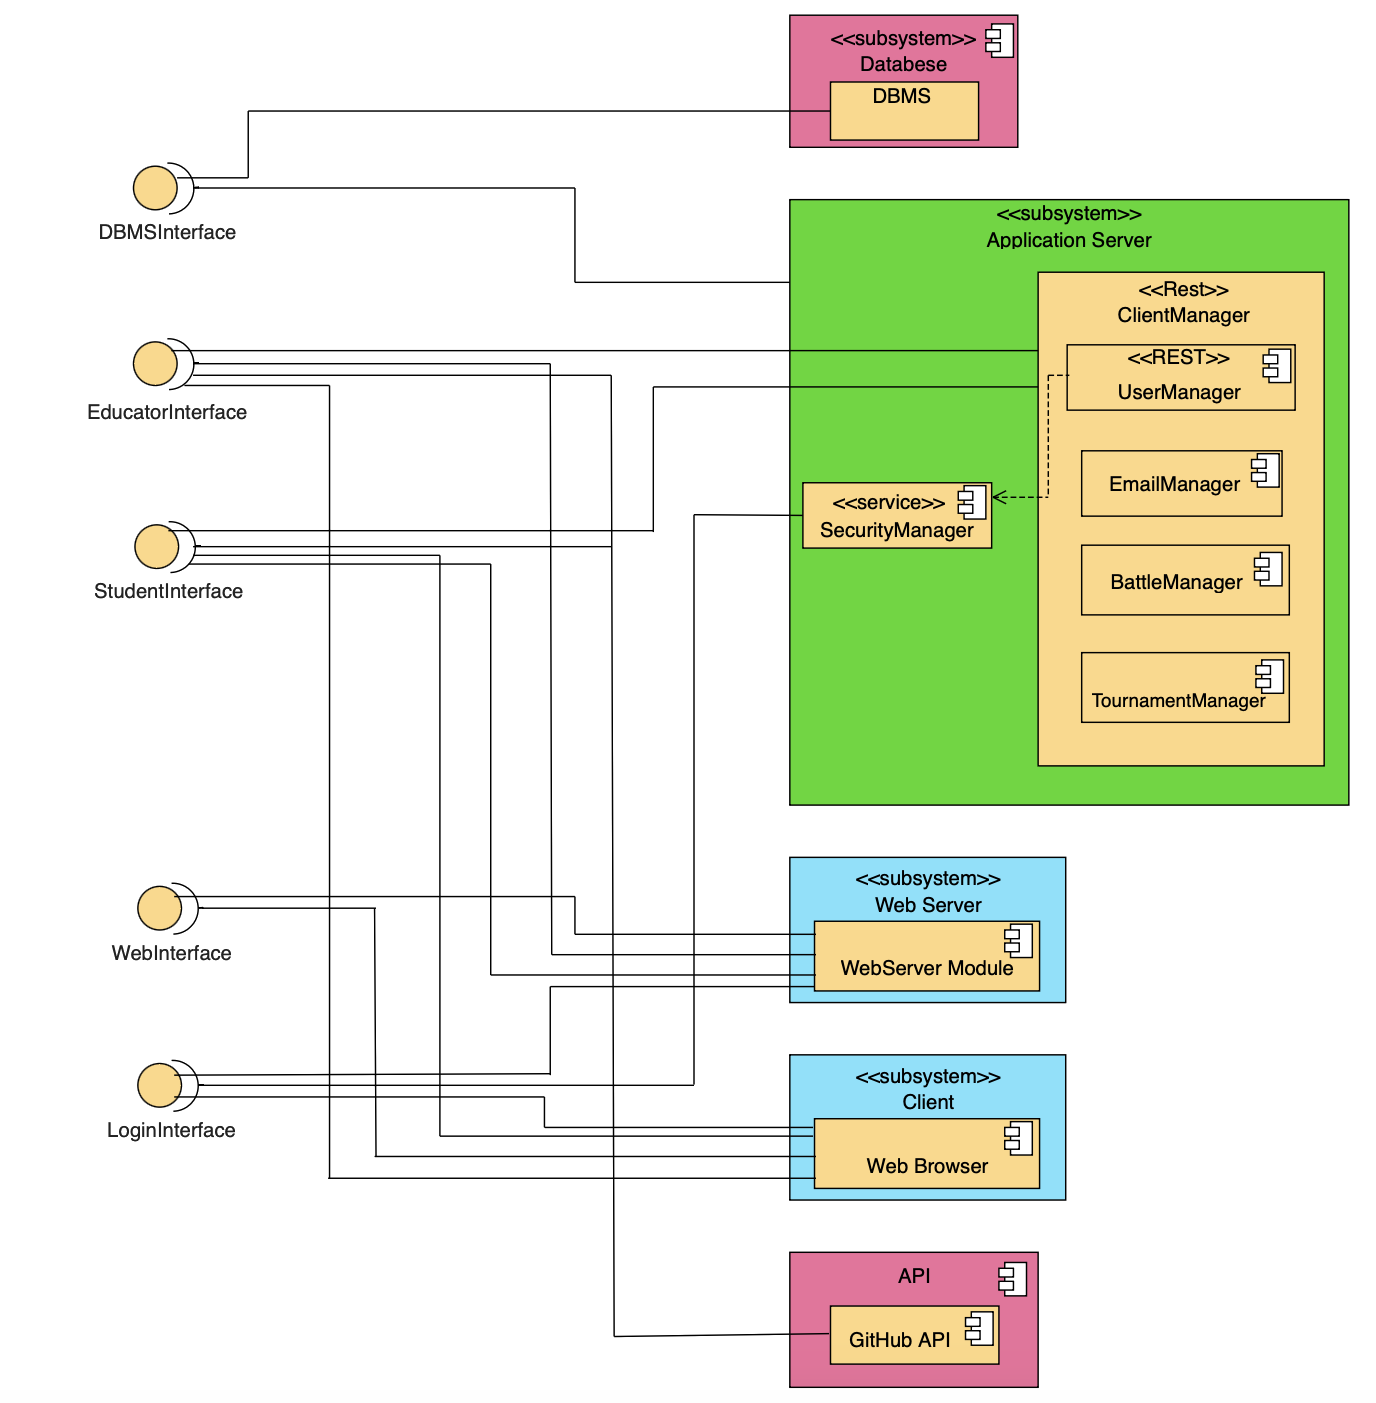
\includegraphics[width=1\linewidth]{Images/Diagrams/ComponentDiagram.png}
    \caption{Component Diagram}
    \label{fig:enter-label}
\end{figure}

\pagebreak

\begin{flushleft}The component diagram, depicted in [Fig. 1], provides a detailed representation of the previously described layers. The web server is responsible for directing browser requests to the application server and returning its corresponding responses.
\end{flushleft}

\begin{itemize}
    \item \textbf{Client Manager} The main module that oversees client requests, initially presenting a landing page where users can choose to either log in or sign up. Upon successful login, the module dynamically displays the interface corresponding to the user's role, showcasing either the educator interface or, if a student is logged in, the student interface.

    \item \textbf{User Manager} This module contains all the features related to the user side, such as log in and sign up and other services like info retrieving and many more.
    
    \item \textbf{Battle Manager} This module contains all the functionalities required to handle interactions with battles inside the platform. It incorporates features such as battle creation and evaluation.

    \item \textbf{Tournament Manager} This module contains all the functionalities required to handle interactions with tournaments. It incorporates features such as tournament joining and badge awarding.

    \item \textbf{Email Manager} This component handles the email notifications which the educators send to the students to join the tournaments.

    \item \textbf{Security Manager} This component is responsible for addressing the security concerns of the S2B system. Its primary objective is to authenticate and authorize requests, relying on tokens provided by clients for verification.
    
\end{itemize}

\clearpage

\subsection{Deployment View}

\begin{figure}[htbp]
    \centering
    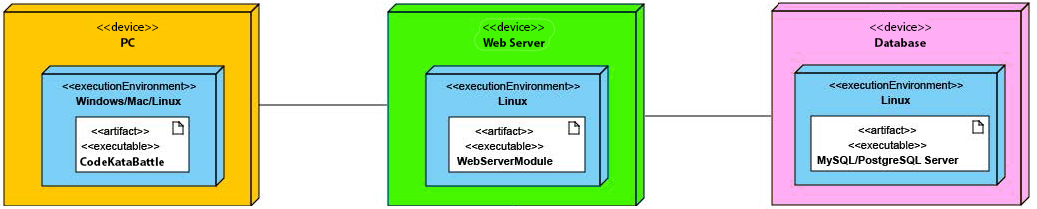
\includegraphics[width=1\linewidth]{Images/Diagrams/Architecture.png}
    \caption{Architecture Diagram}
    \label{fig:enter-label}
\end{figure}

\begin{flushleft}
The deployment diagram, illustrated in [Fig. 2], delineates the platform's components, excluding the GitHub API, which facilitates code uploading interactions. Each component operates within its designated Operating System. The identified tiers are as follows:    
\end{flushleft}

\begin{itemize}
    \item \textbf{Tier 1:} The client computer (student or educator) with a web browser installed.
    \item \textbf{Tier 2:} The web servers exclusively handle incoming client requests without engaging in computational tasks. Their primary function is to route these requests to the application servers and furnish the client with an HTML file. The client then assembles the page using client-side scripting, incorporating stylistic elements from CSS sheets.
    \item \textbf{Tier 3:} The application server serves as the primary executor of the S2B system, hosting the core functionalities within its application layer. Communication with the client tier is established through APIs accessed by the web servers. Ultimately, connectivity to the data tier is facilitated through the DBMS gateway.
    \item \textbf{{Tier 4:}} The DBMS servers store and execute actions on data as directed by instructions from the application servers.
\end{itemize}

\subsection{Runtime View}
In this segment, the diagrams exclusively depict the runtime view aligned with the use cases outlined in the Requirements and Specifications Document (RASD). These runtime views illuminate the dynamic interactions among the different components, illustrating how CodeKataBattle executes its functionalities.

\clearpage

\subsubsection{User Registration}
This sequence diagram illustrates the process initiated when a user wants to register on the CodeKataBattle (CKB) platform. The user begins by selecting whether to register as a student or an educator. Subsequently, the system transmits the user's credentials to the UserManager component, which, in turn, dispatches these credentials to the EmailController. The EmailController assumes the responsibility of sending an email confirmation to the user. Simultaneously, the credentials are forwarded to the Database Management System (DBMS) for verification. Ultimately, a message indicating the validity or invalidity of the credentials is relayed back to the platform.

\begin{figure}[htbp]
    \centering
     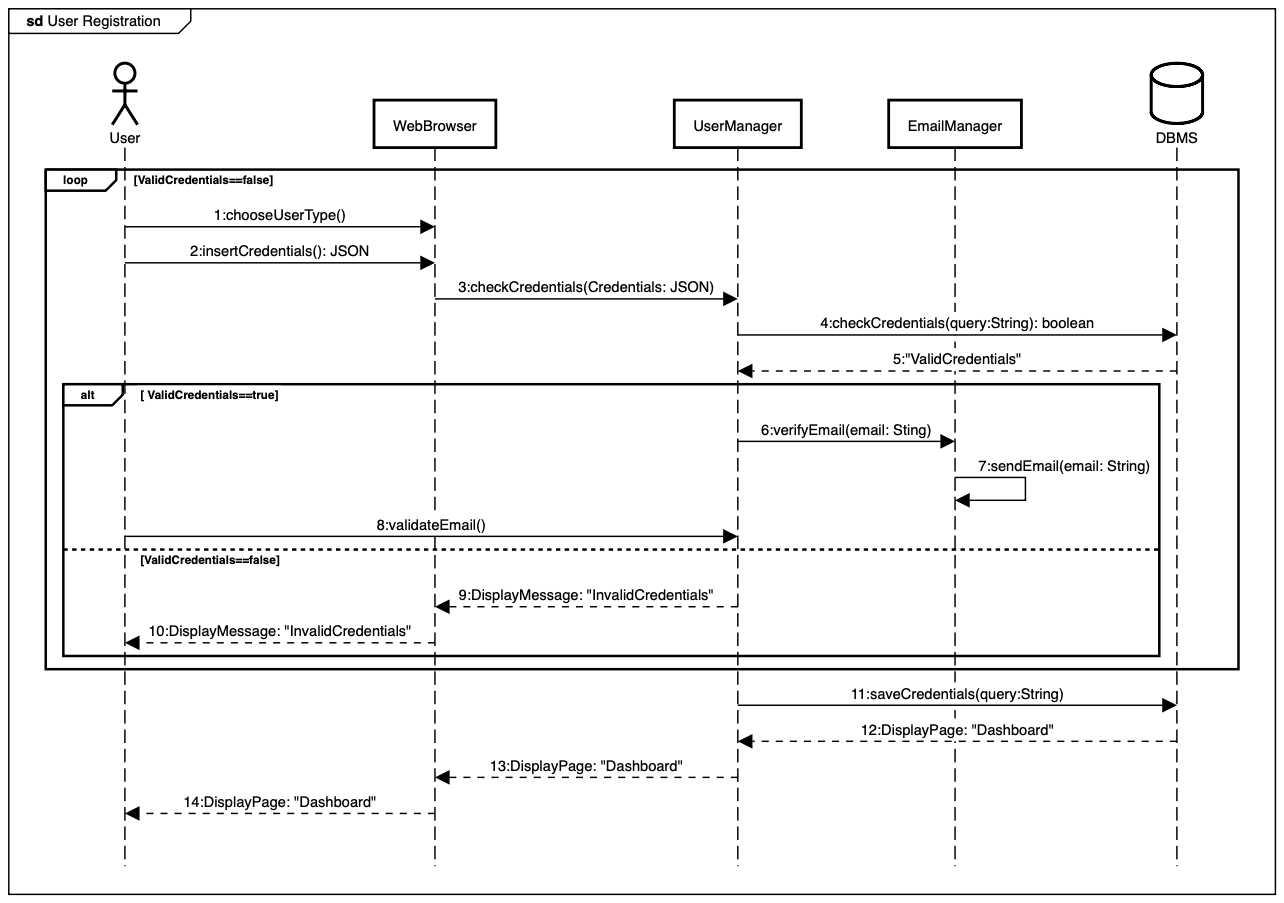
\includegraphics[width=1\linewidth]{Images/Sequence Diagrams/UserRegistration.png}
    \label{fig:enter-label}
\end{figure}

\clearpage

\subsubsection{User Login}
This diagram illustrates the login process on the CodeKataBattle Platform (CKB). The user begins by entering credentials, which the system then forwards to the UserManager. Subsequently, the UserManager checks the provided credentials with the Database Management System (DBMS) to verify their accuracy. If the credentials are correct, a validation message is sent back, granting the user access to the platform. Otherwise, if the credentials are incorrect, an error message is dispatched, denying access.

\begin{figure}[htbp]
    \centering
    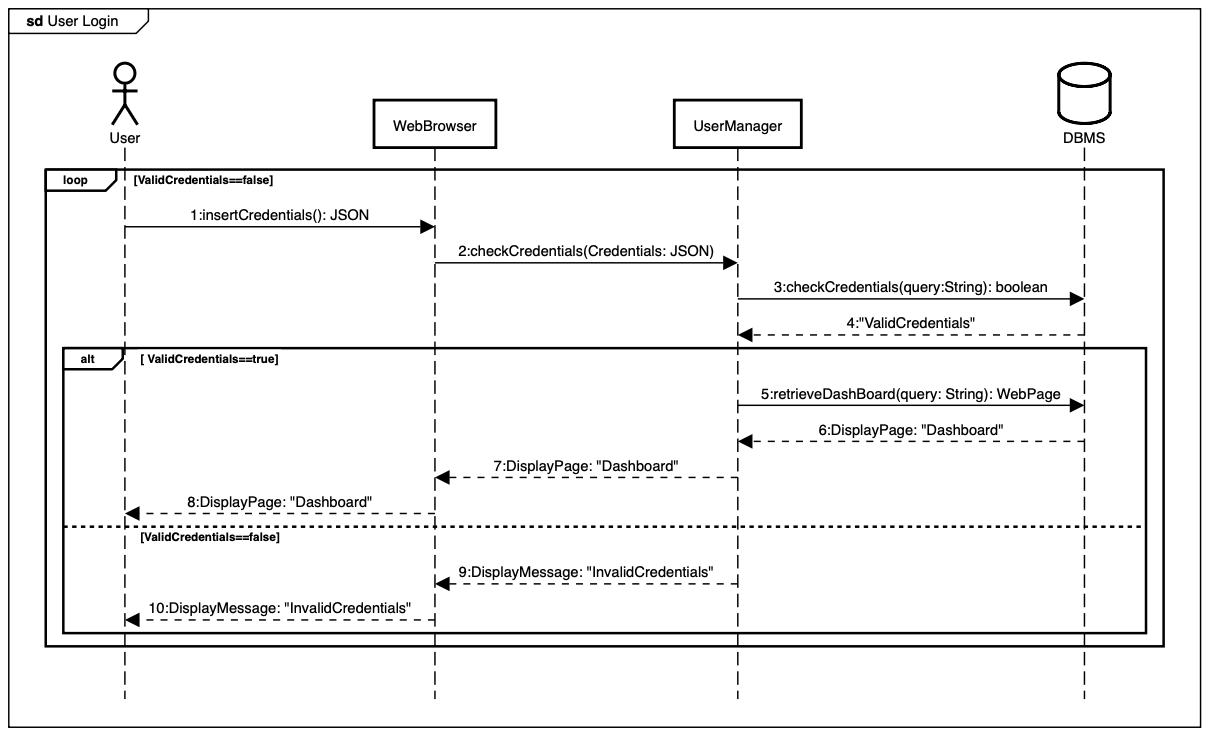
\includegraphics[width=1\linewidth]{Images/Sequence Diagrams/UserLogin.png}
    \label{fig:enter-label}
\end{figure}

\clearpage

\subsubsection{Educator creates a tournament}
This diagram outlines the process through which an educator creates a new tournament. The educator begins by selecting a name, and through the TournamentManager and DBMS, the system checks for name availability, sending a corresponding message. Following this, the educator specifies the registration deadline, validating it through the TournamentManager against criteria such as being after the date of creation, with a message indicating the validity sent back.
$\\$Next, the educator designates the programming language for the tournament, and this information is stored in the DBMS through the TournamentManager, with an acknowledgment sent in return. Subsequently, the educator may grant access to colleagues by entering their email addresses. The EmailManager checks the DBMS for the email's existence, and upon finding a match, sends out an invitation. A message confirming access is then sent back.
$\\$Lastly, the educator defines badges, with the option to create new ones or use existing ones. The system processes this information and sends a confirmation message, acknowledging the successful completion of the tournament creation process.

\begin{figure}[htbp]
    \centering
    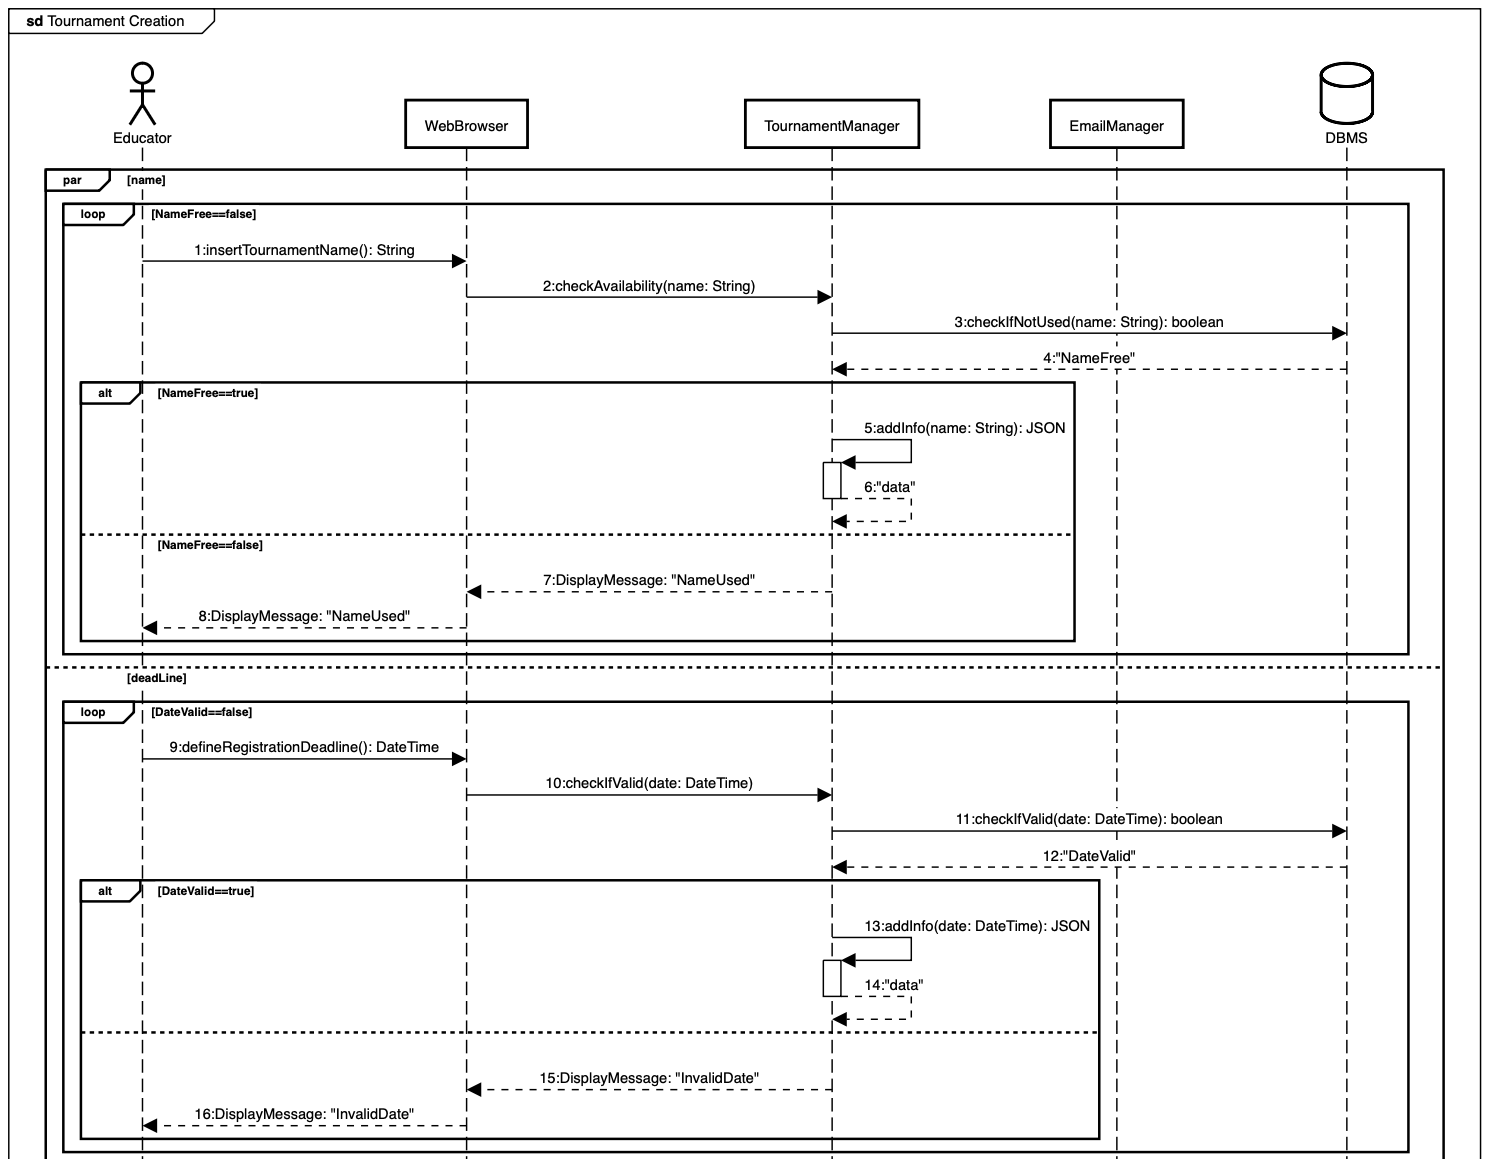
\includegraphics[width=1\linewidth]{Images/Sequence Diagrams/TournamentCreation1.png}
    \label{fig:enter-label}
\end{figure}

\begin{figure}[htbp]
    \centering
    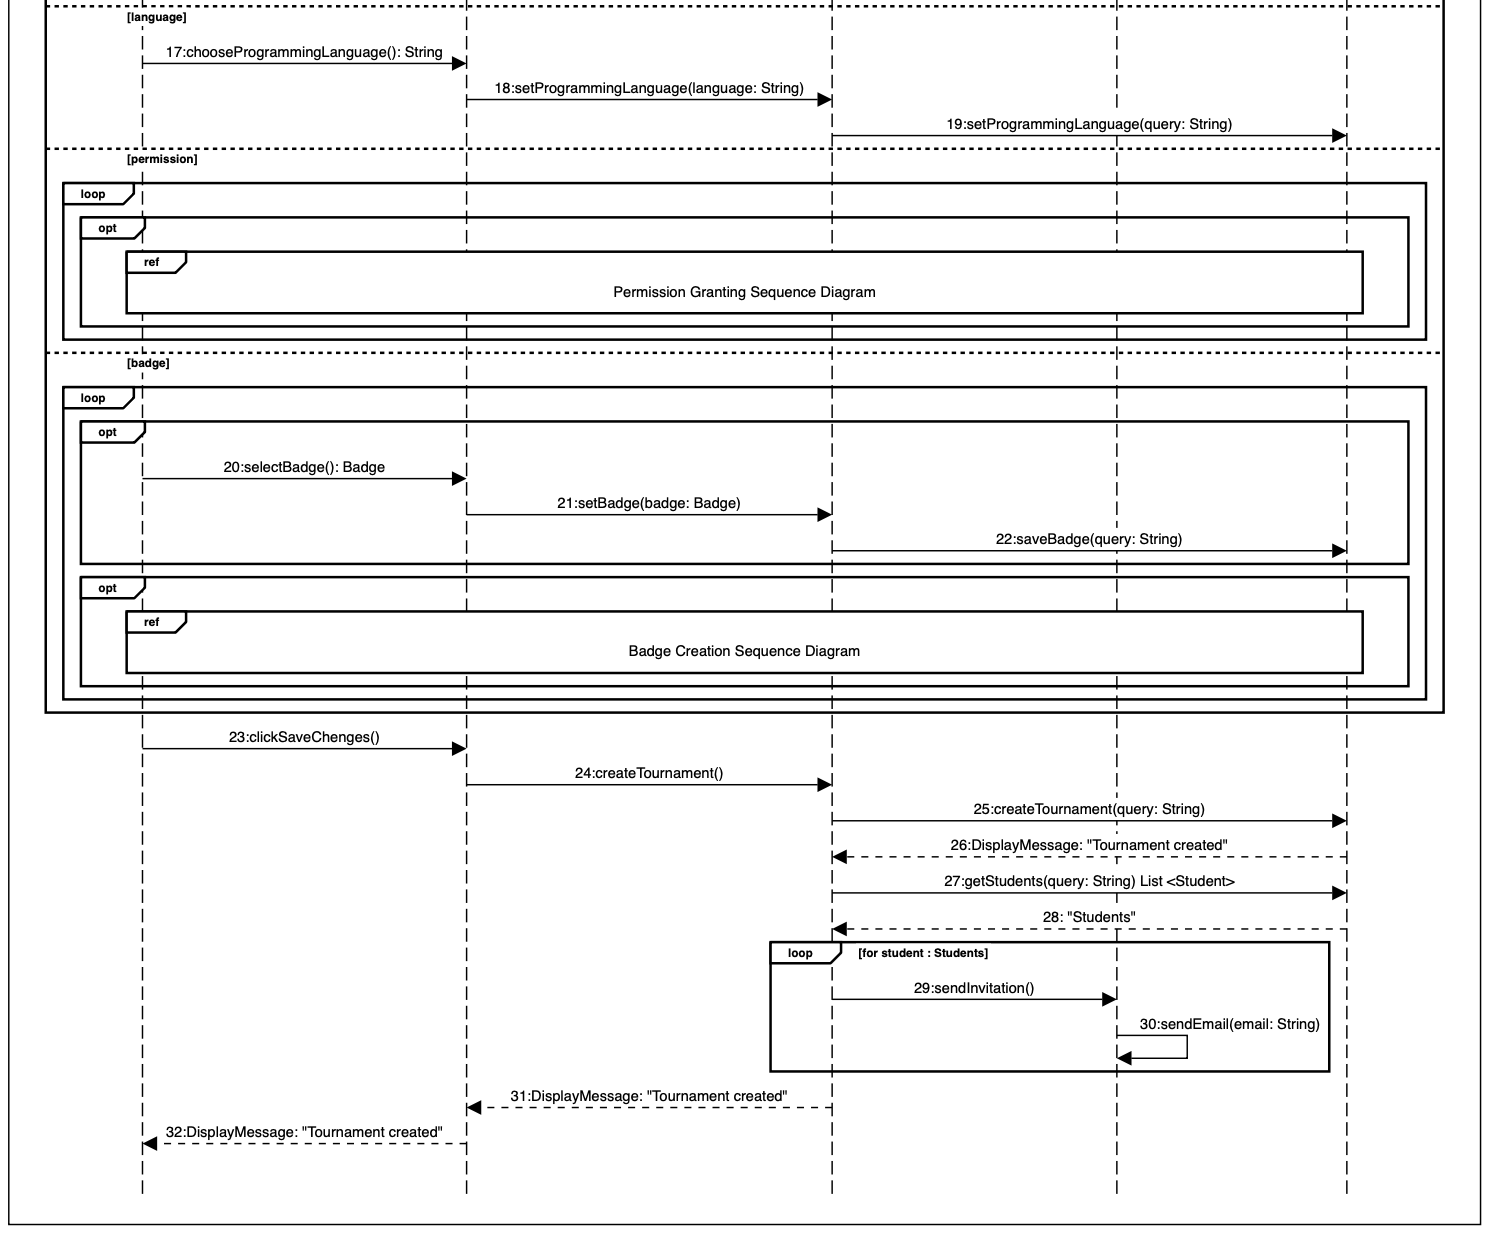
\includegraphics[width=1\linewidth]{Images/Sequence Diagrams/TournamentCreation2.png}
    \label{fig:enter-label}
\end{figure}

\clearpage

\subsubsection{Educator creates a badge}
This sequence diagram outlines the process wherein an educator creates a badge. The educator initiates the process by entering a name for the badge. The system then forwards the name to the UserManager, which, in turn, checks its availability in the Database Management System (DBMS). If the name is already in use, an error message is returned to the system; otherwise, a confirmation message is dispatched.
$\\$Following this, the educator proceeds to define new rules or utilize existing ones for badge acquisition. In both scenarios, a confirmation message is relayed back. Subsequently, the educator is prompted to add variables, and upon completion, a confirmation message is sent.
$\\$Finally, the educator is required to incorporate an icon for the badge. Once this task is accomplished, a confirmation message is issued, signaling the successful completion of the badge creation process.

\begin{figure}[htbp]
    \centering
    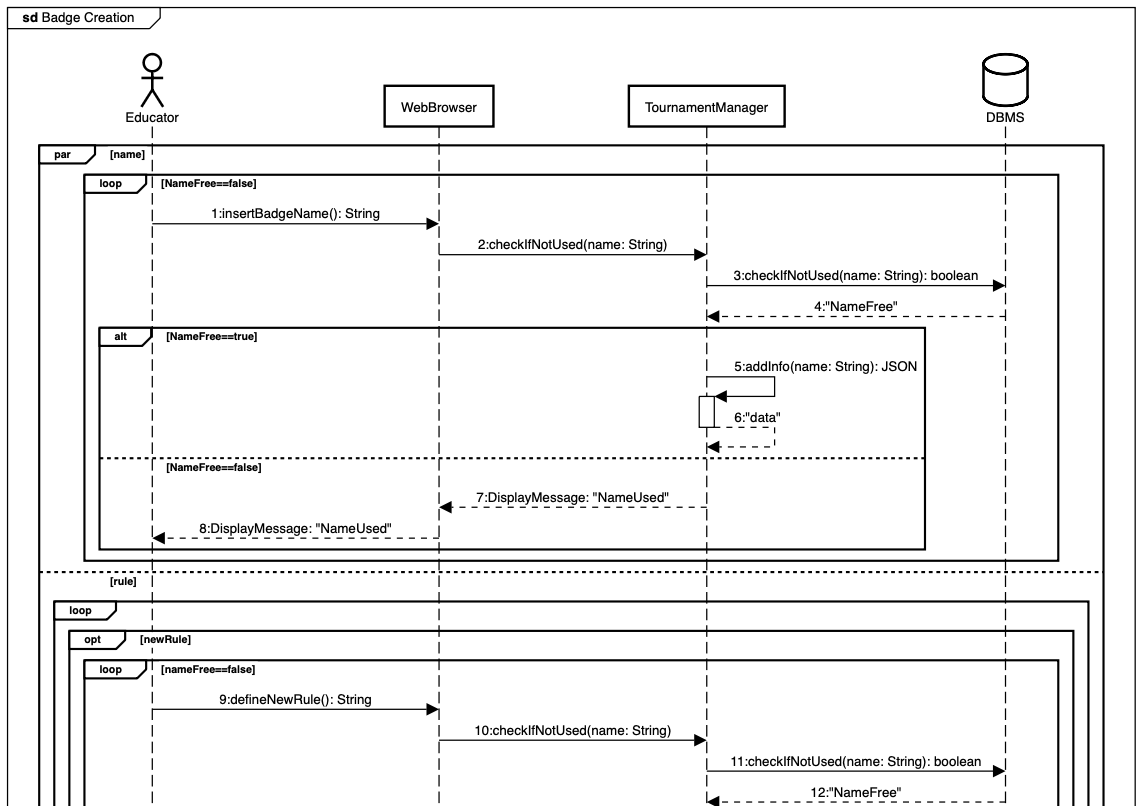
\includegraphics[width=1\linewidth]{Images/Sequence Diagrams/BadgeCreation1.png}
    \label{fig:enter-label}
\end{figure}

\begin{figure}[htbp]
    \centering
    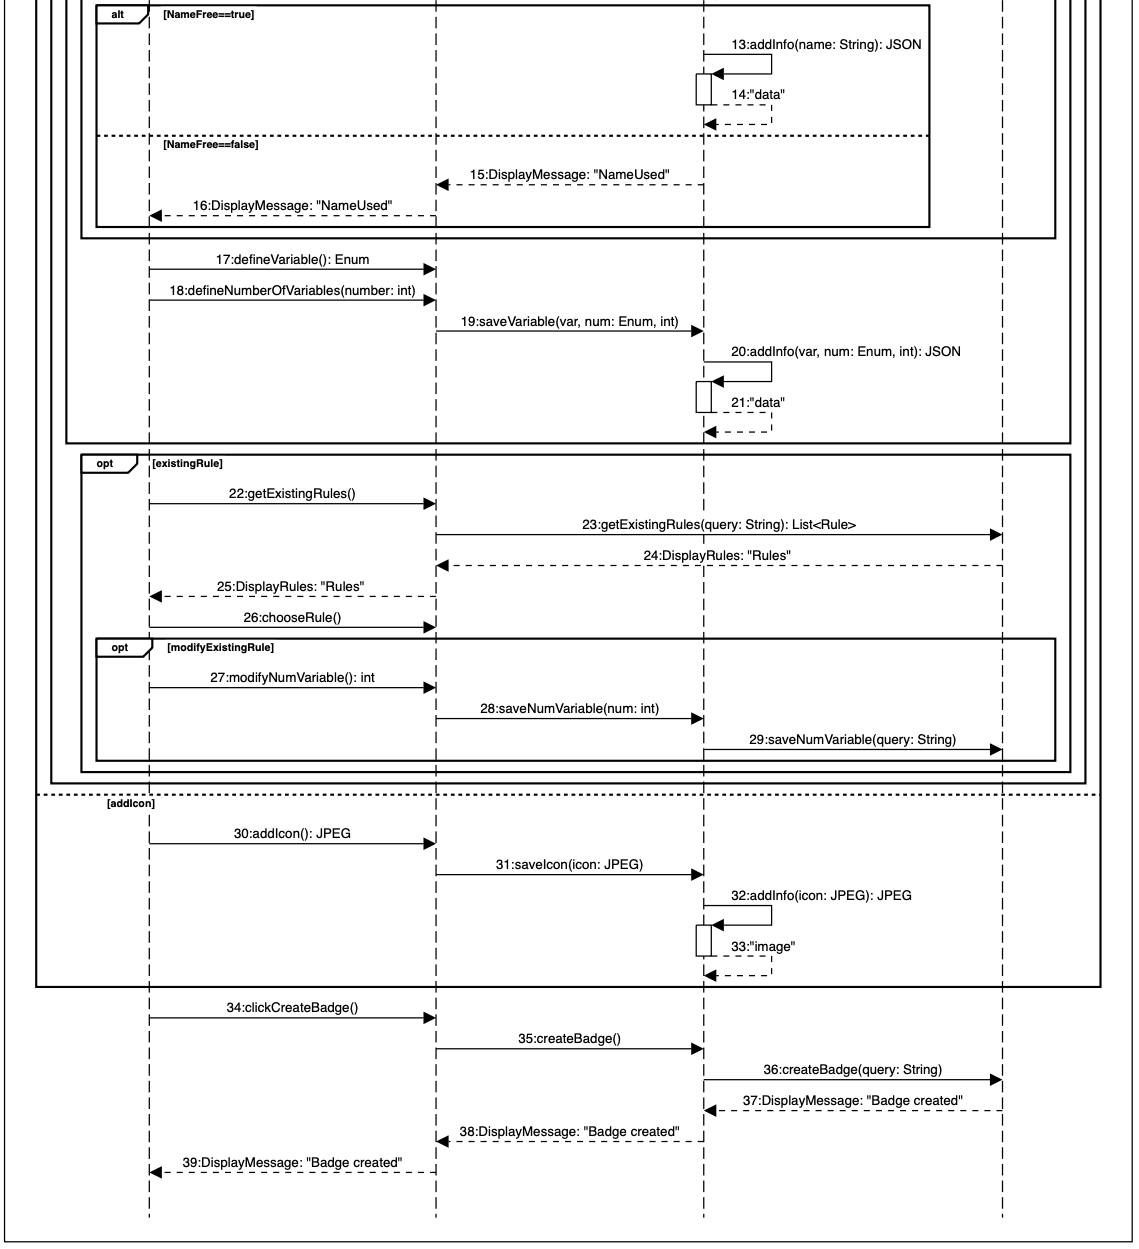
\includegraphics[width=1\linewidth]{Images/Sequence Diagrams/BadgeCreation2.png}
    \label{fig:enter-label}
\end{figure}

\clearpage

\subsubsection{Educator grants permission to a colleague}
This sequence diagram illustrates the steps an educator takes to provide access to a tournament for another educator. The process begins with the educator entering the email address into the system. The system then verifies the email's presence in the Database Management System (DBMS). If the email is found, an acknowledgment is sent to the Email Manager, which subsequently dispatches the invitation. A message confirming access, labeled "Access Granted," is then sent back. In the event that the email is not found in the DBMS, the process remains the same. However, the Email Manager refrains from sending an invitation, and instead, messages indicating "Access Denied" are sent back to signify the unavailability of the email address. 


\begin{figure}[htbp]
    \centering
    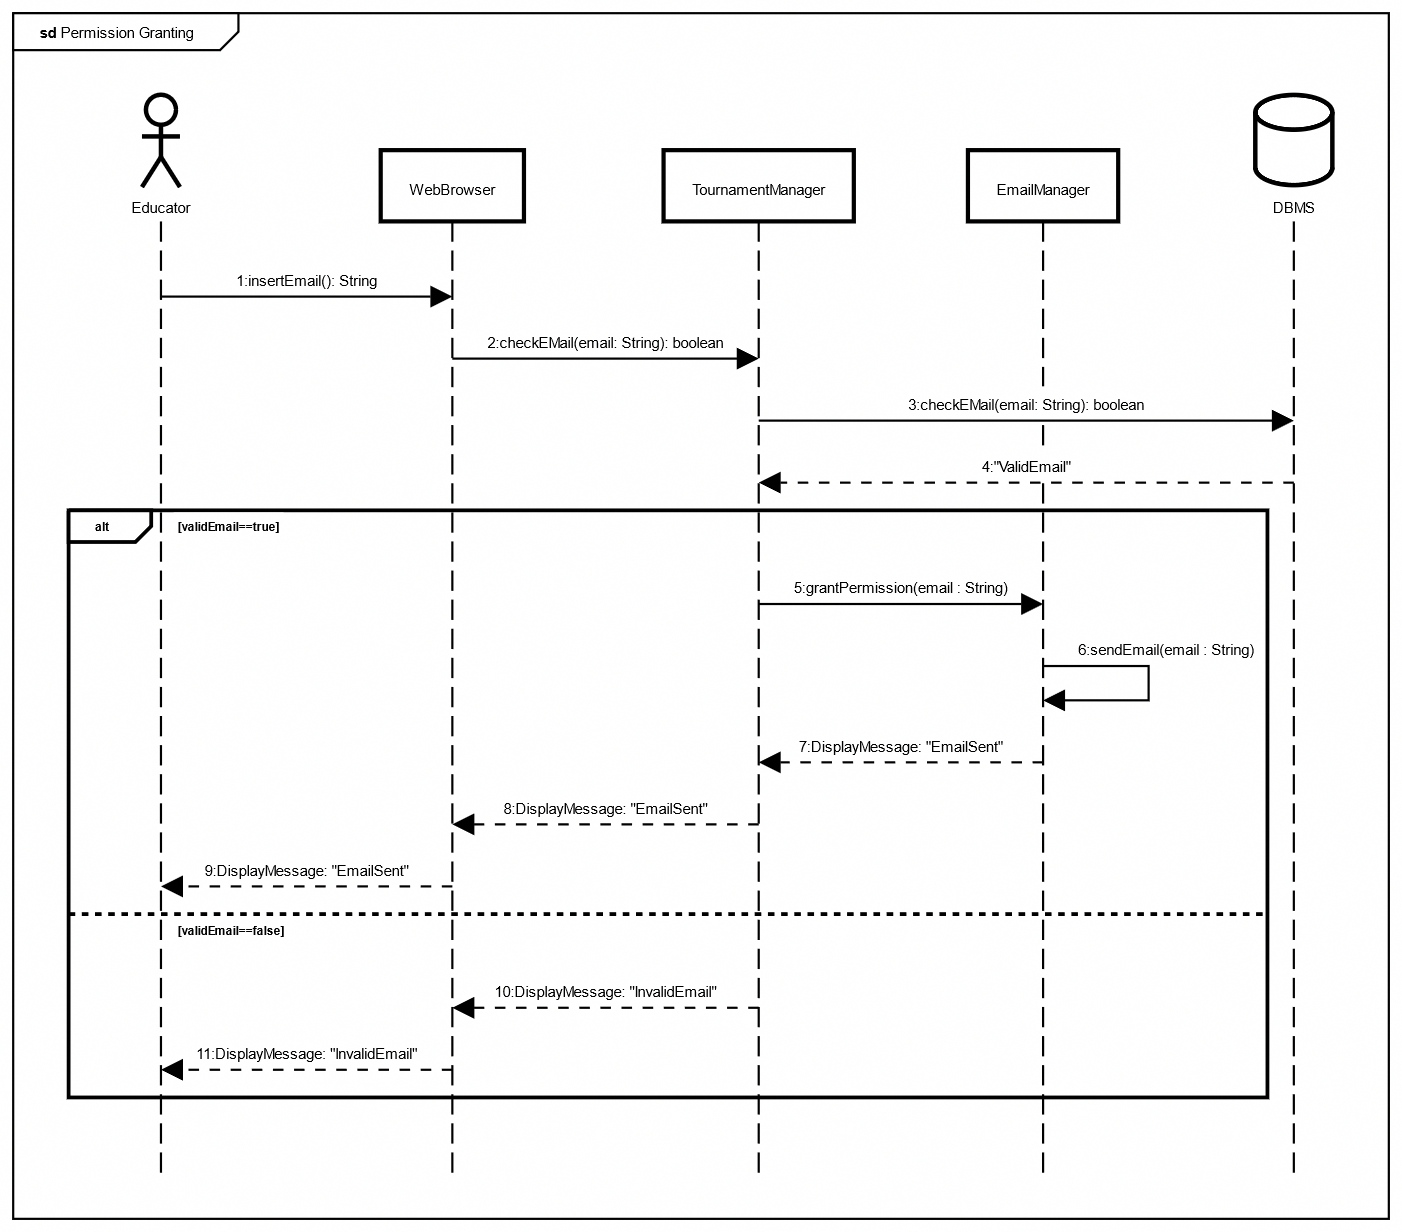
\includegraphics[width=1\linewidth]{Images/Sequence Diagrams/PermissionGranting.png}
    \label{fig:enter-label}
\end{figure}

\clearpage


\subsubsection{Student enrolls in a tournament}
This sequence diagram shows the procedure for the enrolment in a tournament. The process begins with the student clicking on the link he/she received from the platform after the educator created the tournament. The system firstly check if the registration deadline has expired. If the deadline is passed, the student can't join the tournament, and the message "Deadline expired. You can't enroll in the tournament" is shown. Otherwise, if the student is not already enrolled in the tournament, the DBMS adds him/her and a confirmation message is sent. If the student was already enrolled, the message "You are already enrolled in the tournament" is displayed.  

\begin{figure}[htbp]
    \centering
    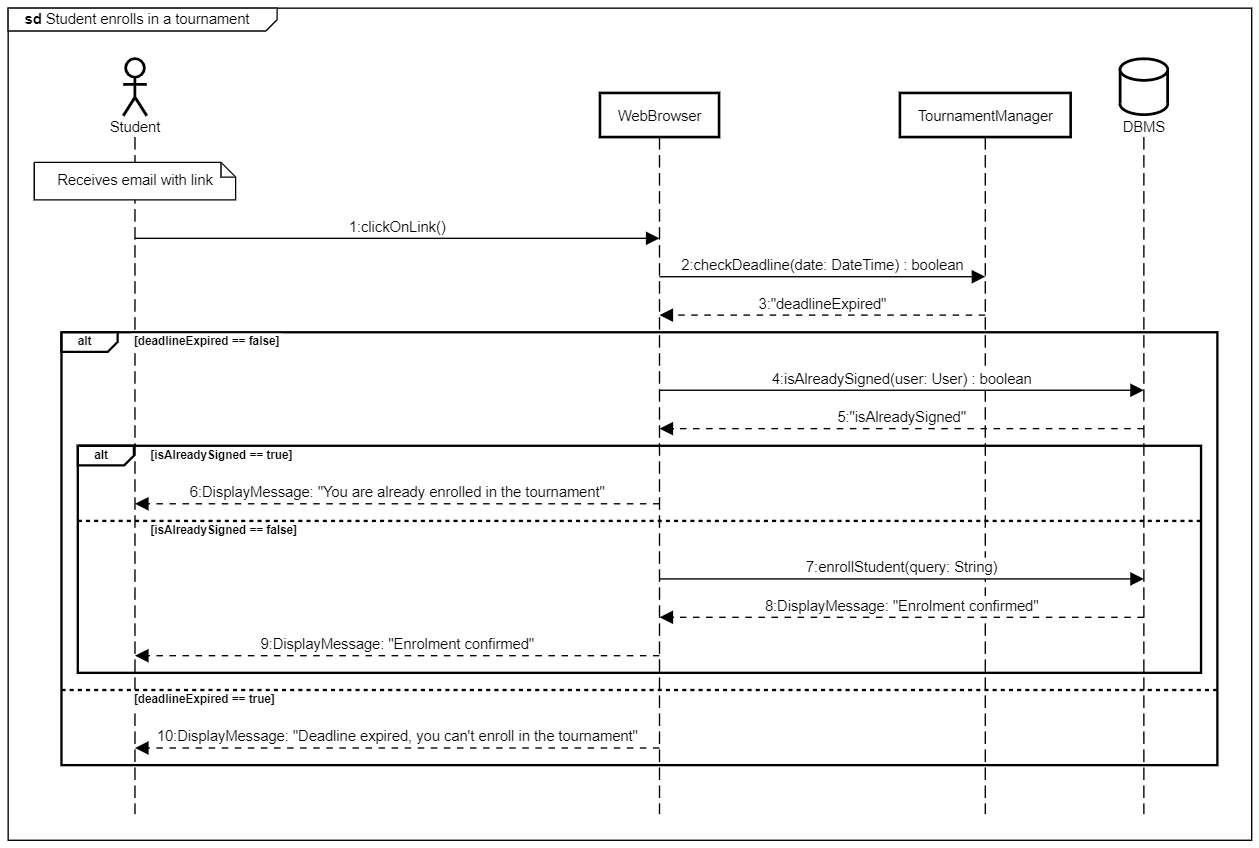
\includegraphics[width=1\linewidth]{Images//Sequence Diagrams/studentEnrollsTournament.png}
    \label{fig:enter-label}
\end{figure}
\clearpage

\subsubsection{Educator creates a battle}
This sequence diagram illustrates the process through which an educator creates a battle. The fields to fill are: battle name, minimum and maximum number of students allowed for each team, a description of the battle, some useful files for the battle and the registration and submission deadlines. Finally, there are three checkboxes for the quality aspects to consider.$\\$
These fields are handled in parallel by the system, which controls their correctness.$\\$
When the educator inserts the battle name, the platform instantly checks whether the name is already used for another battle or not.$\\$
The control on the minimum and maximum number of students checks that the maximum number is greater or equal to the minimum number.$\\$
The system verify that all the required files have been uploaded.$\\$
The control on the deadlines consists in verifying that the dates are not in the past, and that the submission deadline occurs after the registration deadline.$\\$
The quality aspects and the description don't need a correctness control.$\\$
If one of the fields is not correct, the system displays a message that describes the problem it faced. Otherwise, if the input is correct, the information is added to a JSON file, that keeps track of all the fields needed for the creation of the battle.$\\$When all the input are correct and the educator clicks on "create battle", the JSON and the documents uploaded are sent to the DBMS, and the message "Battle created" is returned to the user.
\begin{figure}[htbp]
    \centering
    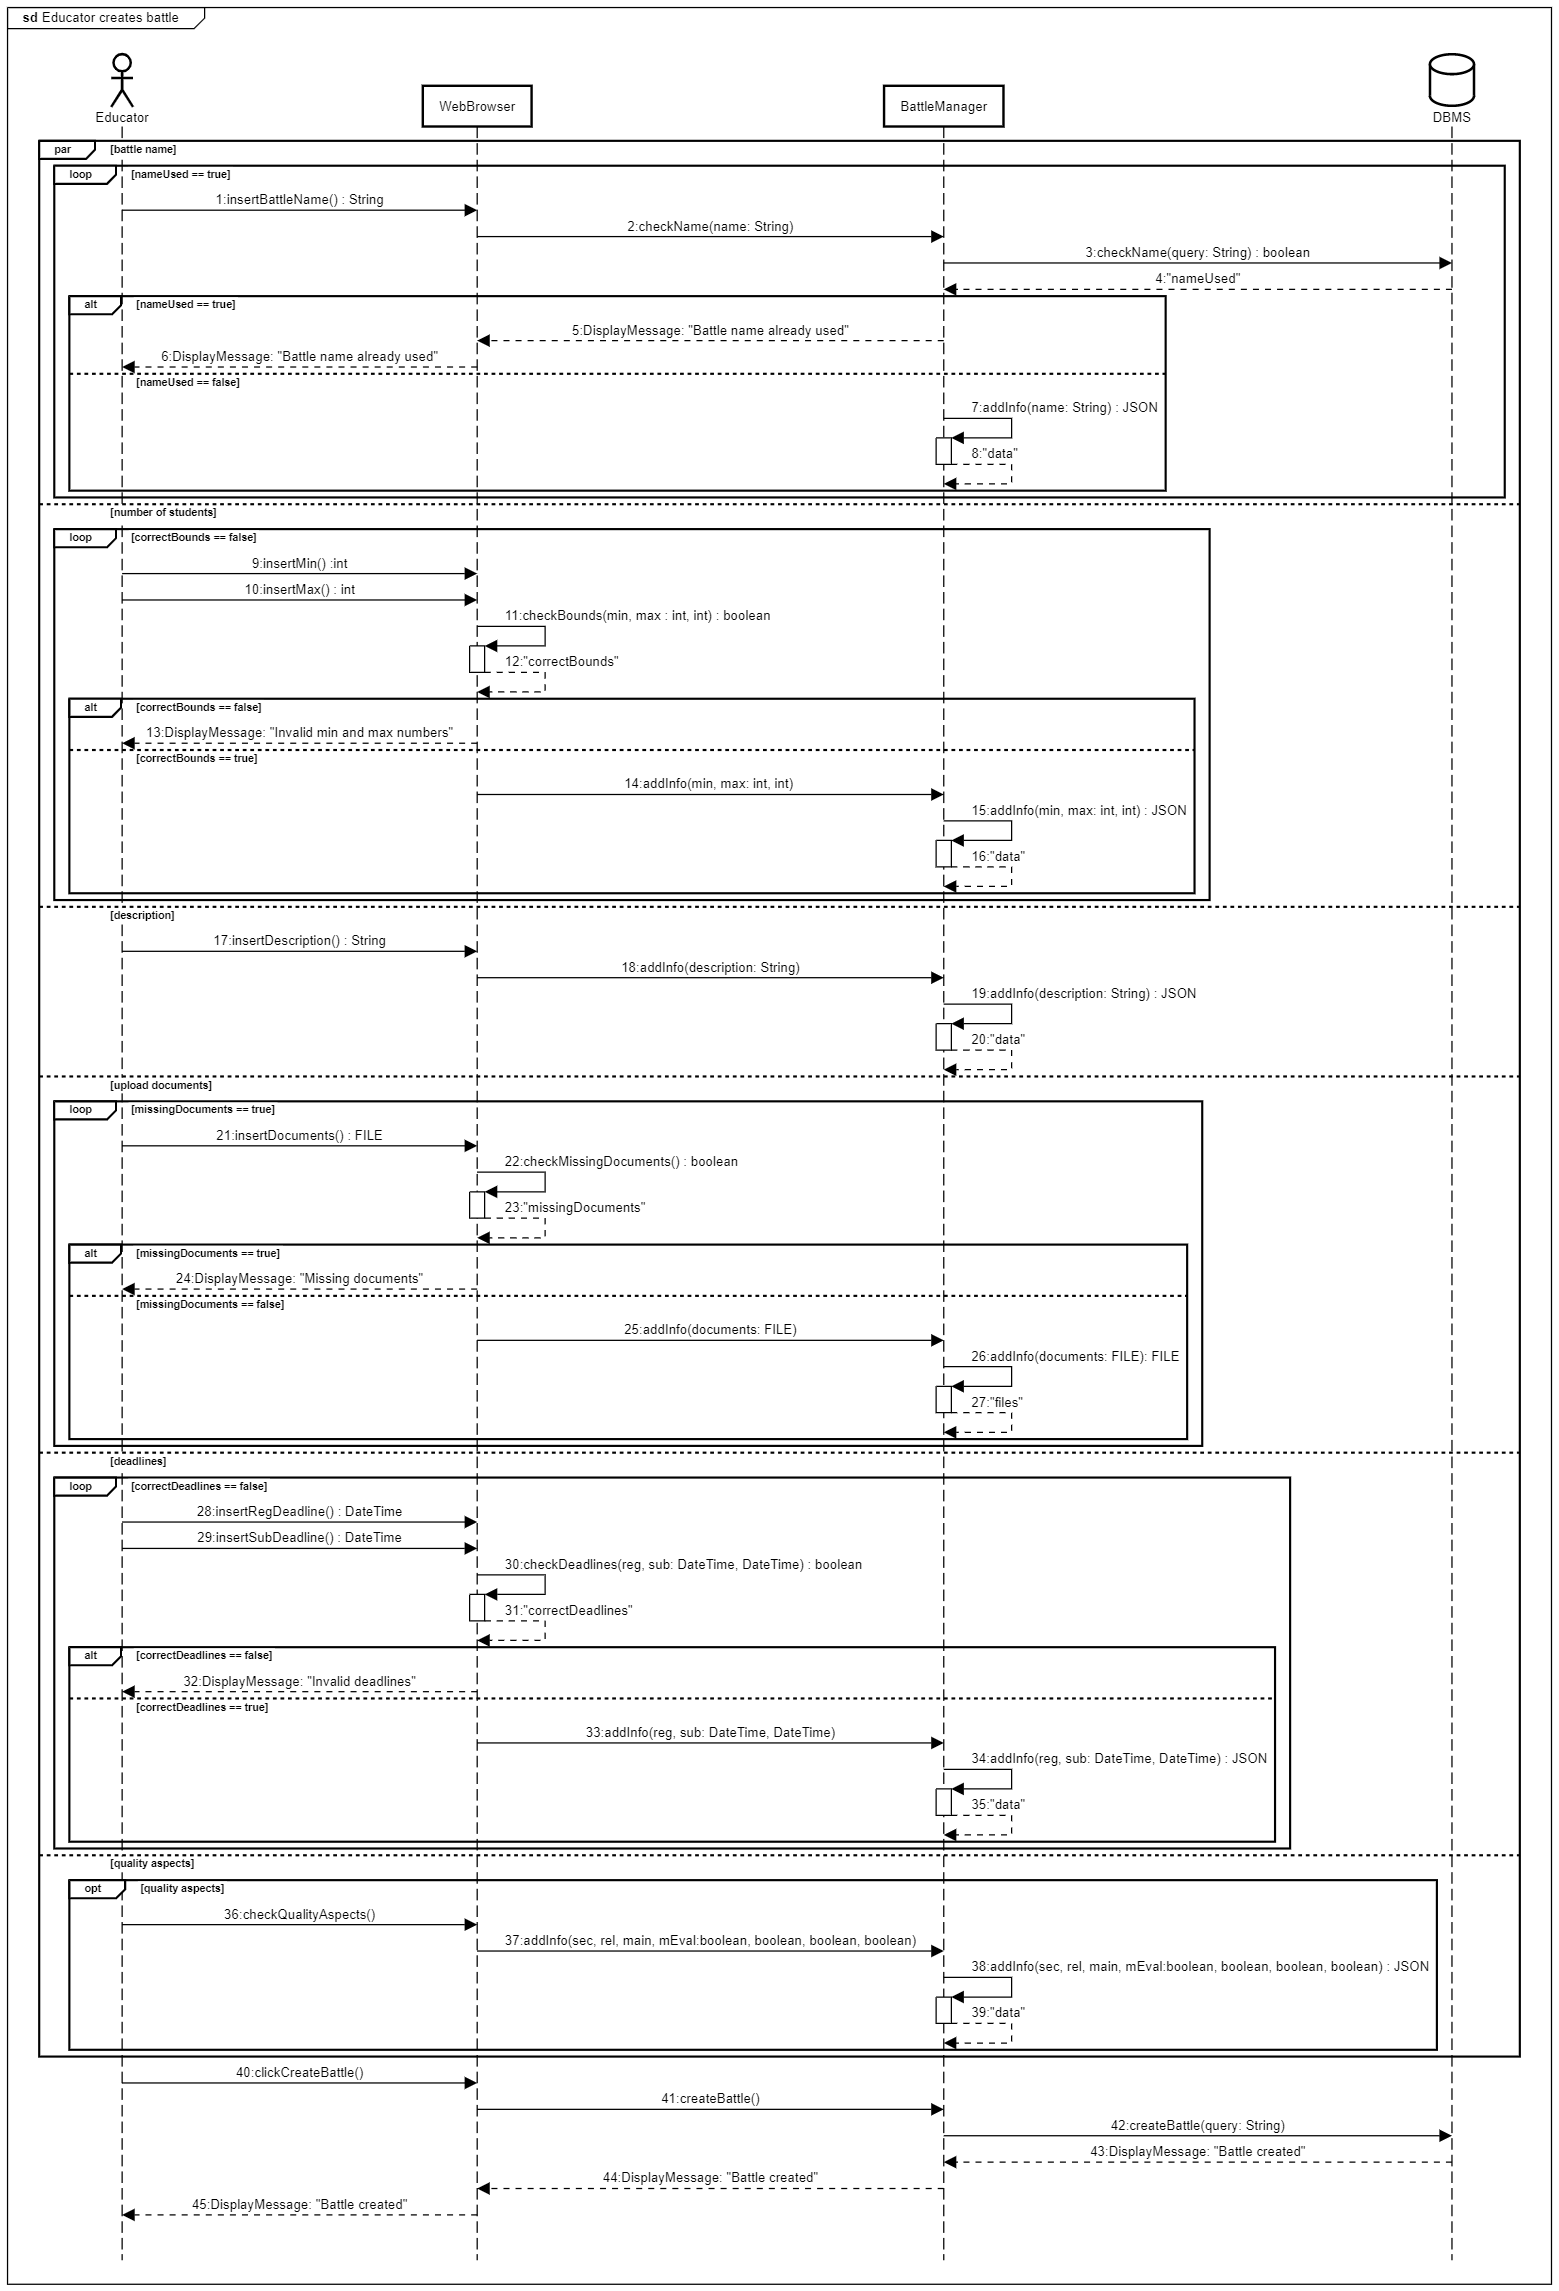
\includegraphics[width=1\linewidth]{Images//Sequence Diagrams/educatorCreatesBattle2.png}
    \label{fig:enter-label}
\end{figure}
\clearpage

\subsubsection{Student enrolls in a battle}
This sequence diagram outlines the procedure wherein a student enrolls in a battle. The first control the system does after the student has clicked on "Join battle" is on the registration deadline. If the deadline is expired, the message "Deadline expired. You can't enroll in the battle" is displayed. Otherwise, the student proceeds selecting the join mode and inserting the name of the team, which is mandatory even if he/she wants to join alone. The system controls if the name has already been taken and, if so, it ask the user to insert a different one until he/she inserts a name that has not been used yet. If the student decided to join with some friends, he/she can insert the emails of his/her colleagues which he/she wants to invite. When an email is inserted, the EmailManager sends the invitation to the friend. The possibility of inserting a new email is based on the minimum and maximum number of students allowed, decided by the educator during the creation of the tournament: if the minimum number of students is not respected, the student has to insert new emails, and when the maximum number is reached, he/she can't insert new emails.
At this point, regardless of the join mode, the student clicks on "join", his/her enrolment is saved in the DBMS and a confirmation message is displayed.

\begin{figure}[htbp]
    \centering
    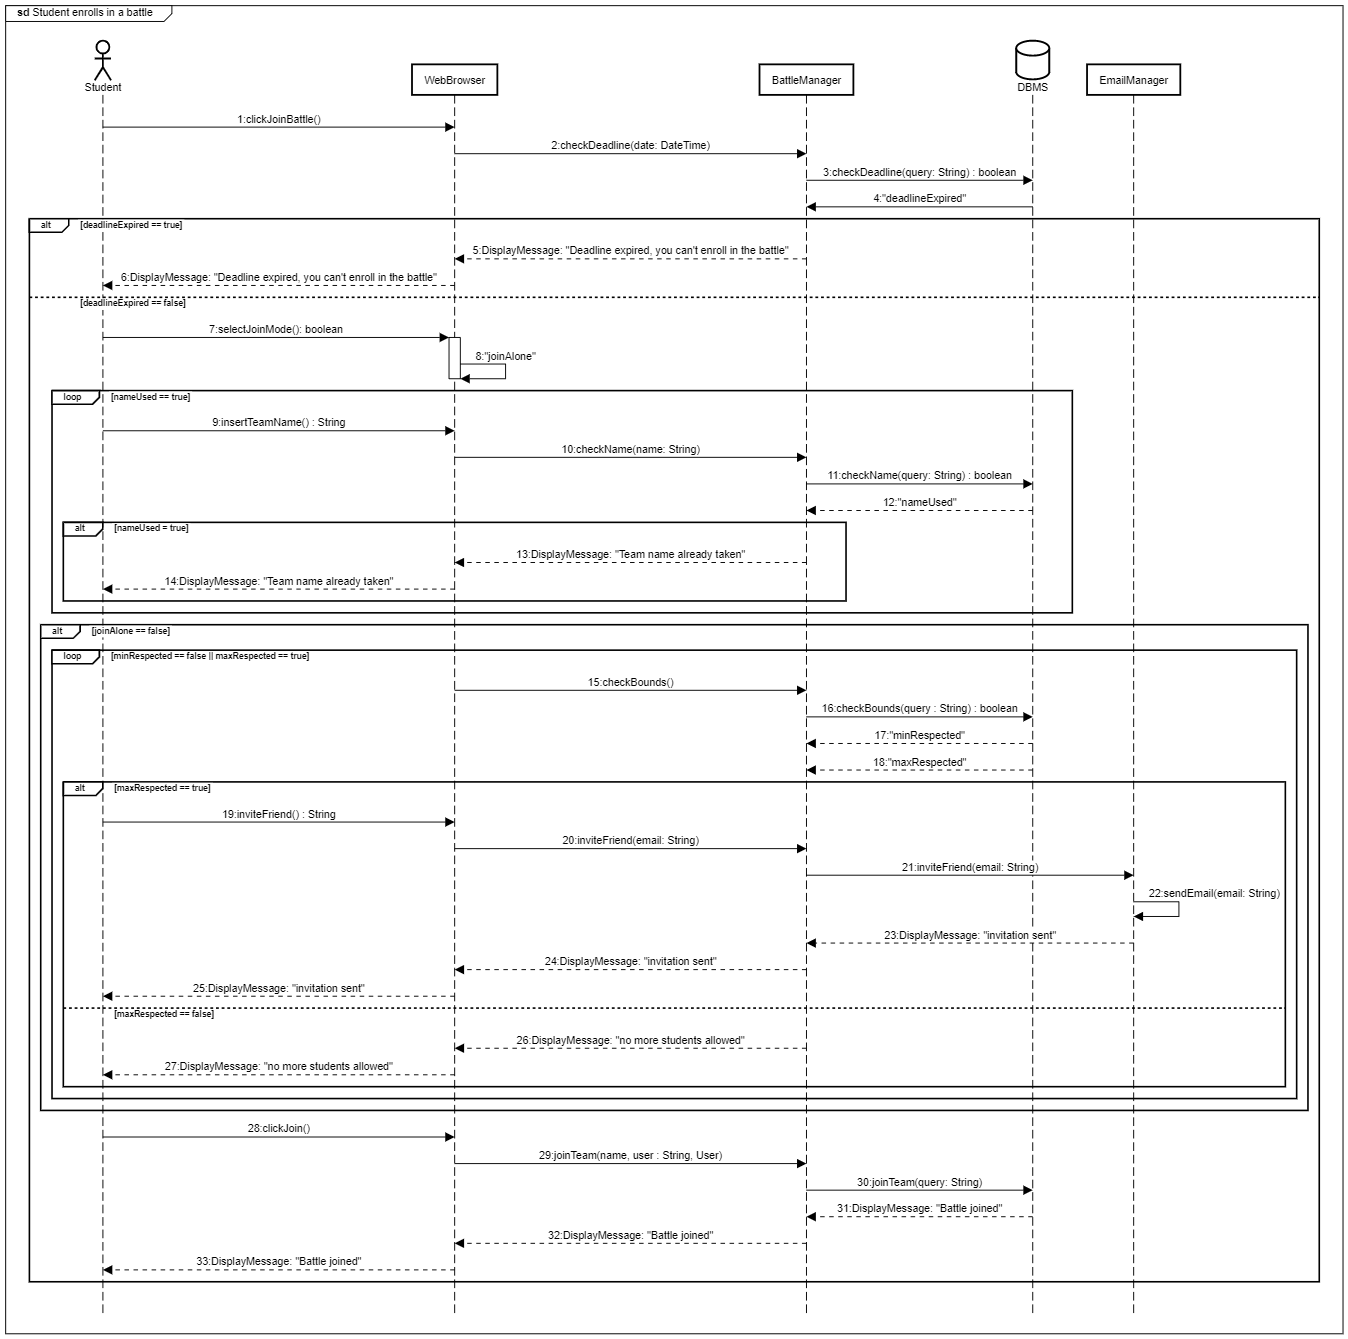
\includegraphics[width=1\linewidth]{Images//Sequence Diagrams/studentEnrollsBattle.png}
    \label{fig:enter-label}
\end{figure}
\clearpage

\subsubsection{Student invites a friend to join his/her team}
This sequence diagram shows the process of invitation in a battle. The student selects the battle he/she is interested in, and the system checks immediately whether other students are allowed or not. If not, the message "no more students allowed is shown", otherwise the student can insert the email of his/her friend. If the email inserted belongs to a student who is already part of another team, the system inform the student that he/she can't invite that user. In case the email doesn't belong to any student already registered in the battle, an invitation email is sent through the Email Manager.

\begin{figure}[htbp]
    \centering
    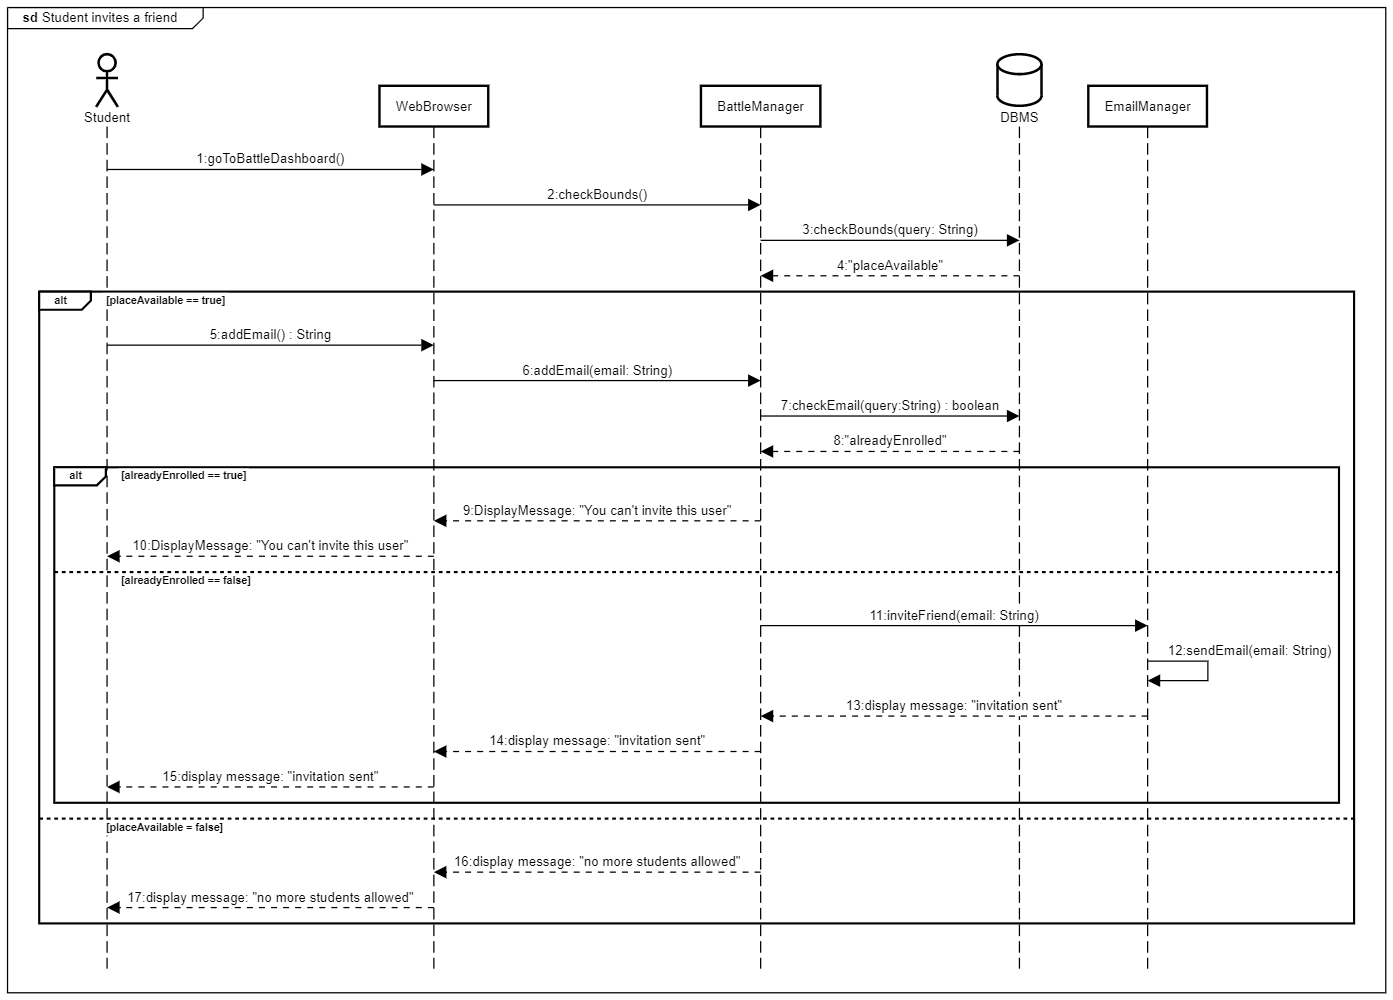
\includegraphics[width=1\linewidth]{Images//Sequence Diagrams/studentInvitesFriend.png}
    \label{fig:enter-label}
\end{figure}
\clearpage

\subsubsection{Student receives an invitation}
This sequence diagram illustrates the process of a student receiving an invitation. Once the invitation link in the email is clicked, the system checks if the registration deadline has expired. If so, the student can't enroll, and a message is shown. Otherwise, the student is signed by the system and saved in the DBMS. 

\begin{figure}[htbp]
    \centering
    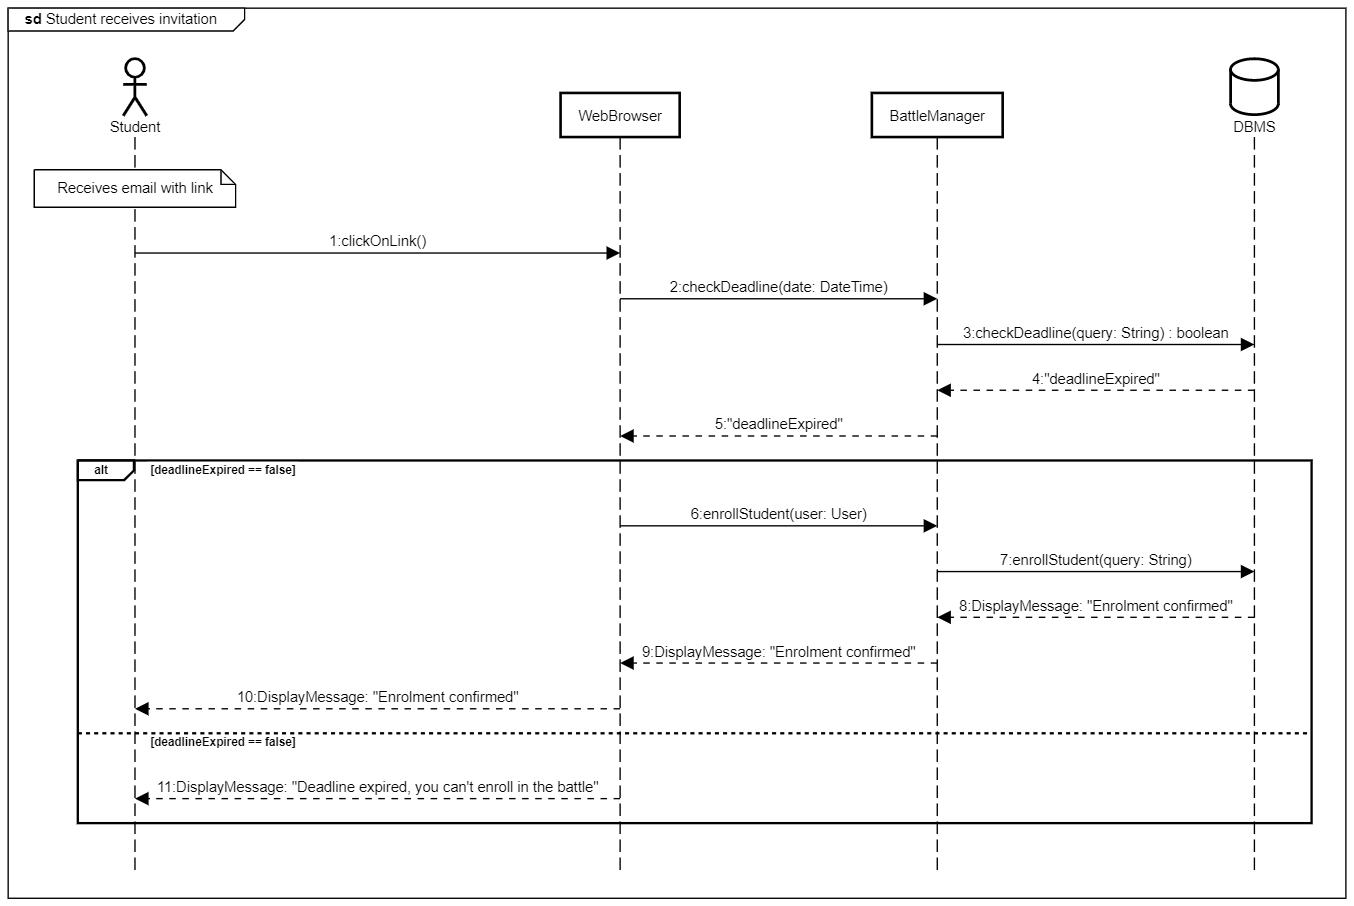
\includegraphics[width=1\linewidth]{Images//Sequence Diagrams/studentReceivesInvitation.png}
    \label{fig:enter-label}
\end{figure}

\clearpage

\subsubsection{Educator evaluates a team's project}
This sequence diagram aims to show the flow of events that occur when an educator evaluates a project, at the end of a battle. The educator starts by clicking on the "Evaluate" button for a specific battle, then the browser forwards the request and the Battle Manager retrieves the battle's information so that the "Evaluation Page" can be shown; if the battle is not finished yet, the educator is presented with an error message. From there, the educator selects which team he/she wants to evaluate and the platform, by accessesing the DBMS, displays him/her the evaluation statistics and current score of the team. Now the educator can optionally check out the GitHub repository or, also optionally, modify the score, which is temporarily stored by the browser. Eventually, the educator must confirm the score and the browser forwards the request to the Battle Manager and DBMS, which acknowledges the request and sends back a confirmation message.
\begin{figure}[htbp]
    \centering
    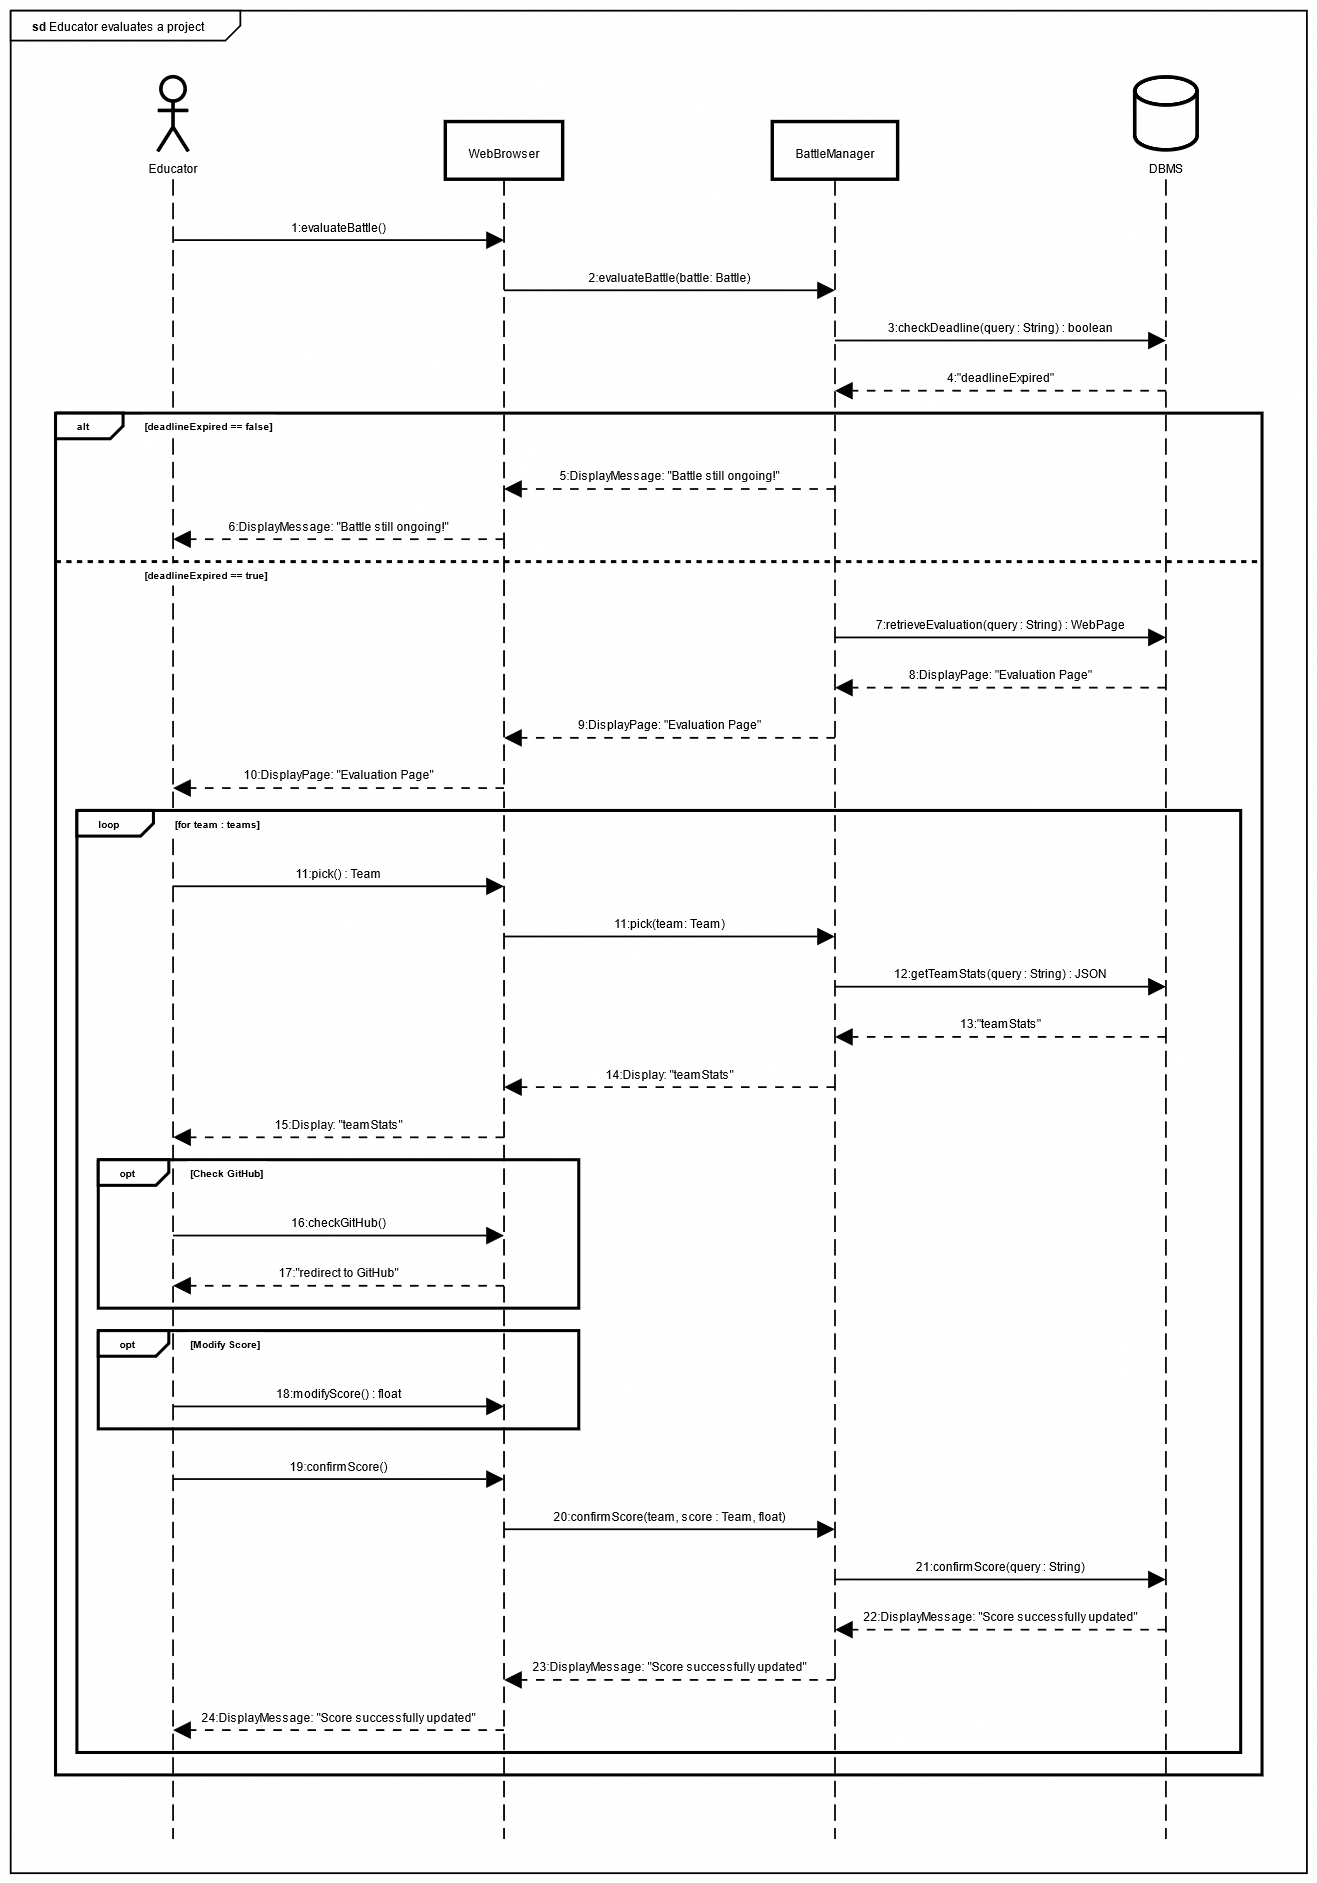
\includegraphics[width=1\linewidth]{Images/Sequence Diagrams/Evaluate.png}
    \label{fig:enter-label}
\end{figure}

\clearpage

\subsubsection{User checks a student profile}
This sequence diagram delineates the procedural flow of events when a user wants to check a student's profile. It starts when the user inputs a username, which is forwarded to the User Manager so that it can be looked up on the DBMS. If the username does not exist in the DBMS, an error message is given back to the Web Browser which displays it to the user. Otherwise, the Web Browser displays the profile corresponding to that username, having retrieved the information by the DBMS. After the user has clicked on the "Show Profile" button, a information request is forwarded to the User Manager, which interrogates the DBMS. Once all the information about the user are gathered, the Web Browser is allowed to redirect to that specific user public profile page, displaying all the information obtained.
\begin{figure}[htbp]
    \centering
    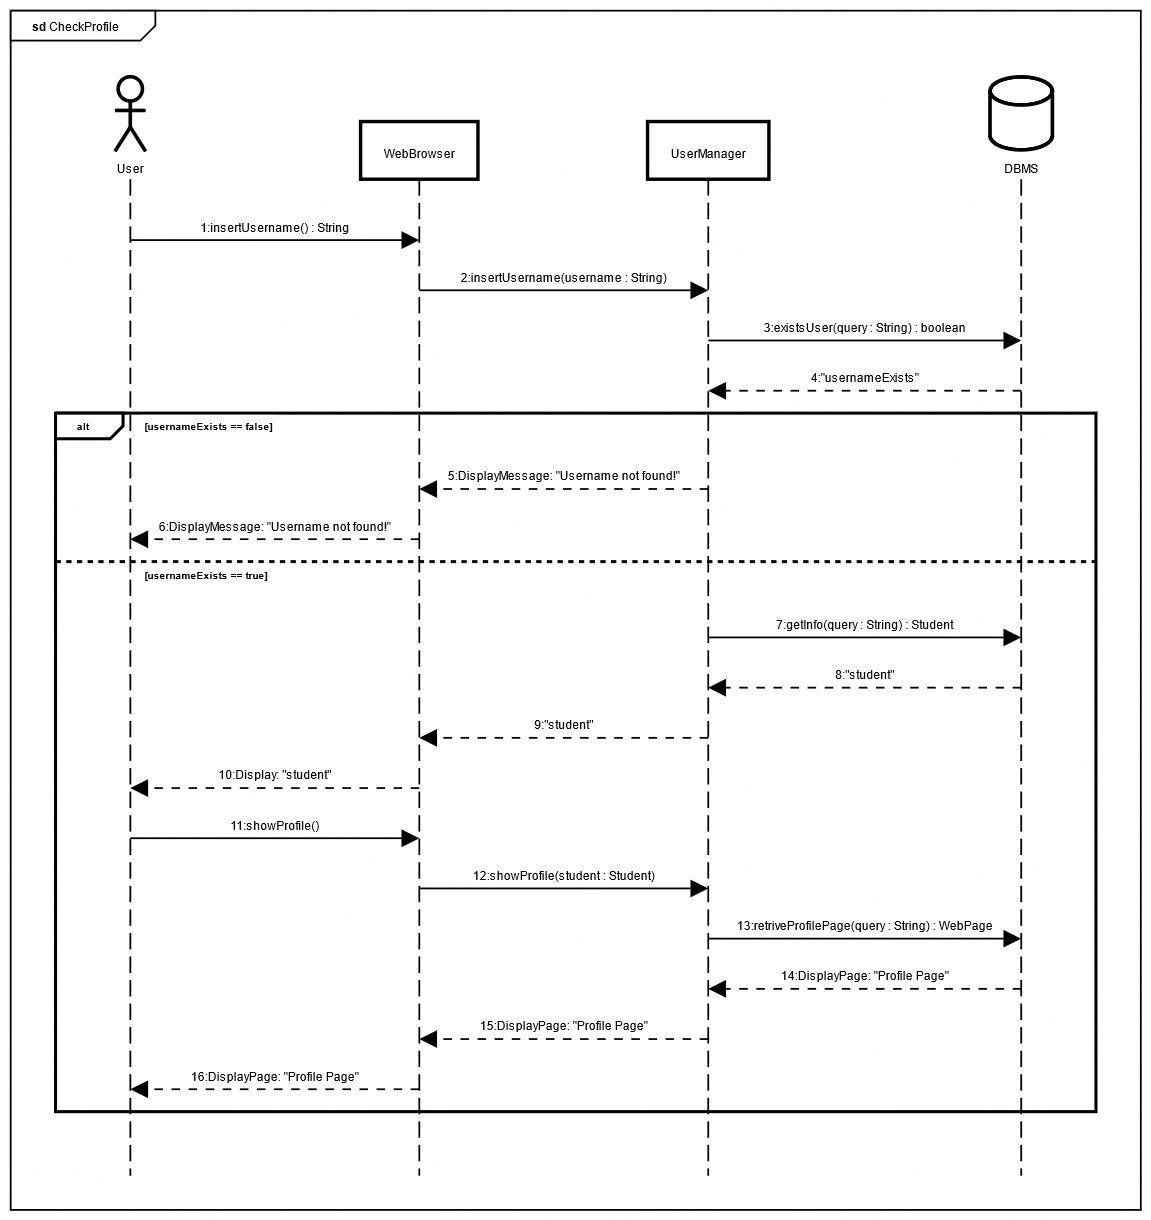
\includegraphics[width=1\linewidth]{Images/Sequence Diagrams/CheckProfile.png}
    \label{fig:enter-label}
\end{figure}

\clearpage

\subsubsection{Student sends a friend request}
This sequence diagram delineates the procedural flow of events of when a student wants to send a friend request to another student. The flow begins with the insertion of the username, which is forwarded to the User Manager so that it can be looked up on the DBMS. If the username does not exist in the DBMS, an error message is given back to the Web Browser which displays it to the student. After gathering the needed information, the Web Browser can display the student's profile to the student looking for it. Lastly, when the student clicks the button to add a friend, the request is transmitted to the DBMS, which acknowledges it and replies back with a confirmation message to the student. 
\begin{figure}[htbp]
    \centering
    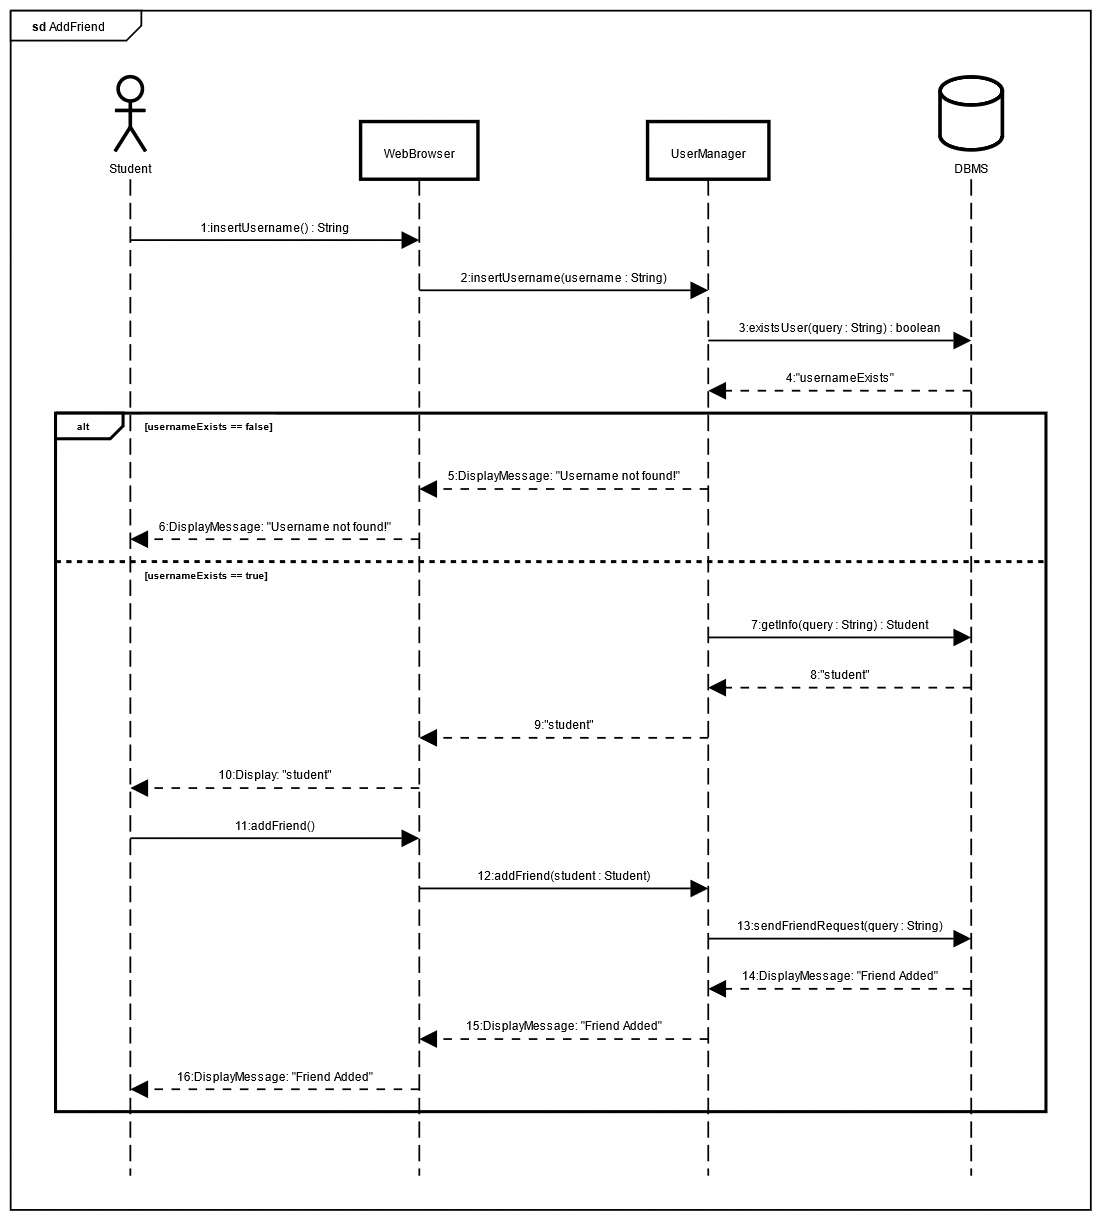
\includegraphics[width=1\linewidth]{Images/Sequence Diagrams/AddFriend.png}
    \label{fig:enter-label}
\end{figure}

\clearpage

\subsubsection{Educator closes a tournament}
This sequence diagram delineates the procedural flow of events when an educator wants to close a tournament. First of all, the educator clicks on the "Close" button and the closeTournament request if sent to the Tournament Manager, so that it can retrieve all the battles inside of it. The Tournament Manager then proceeds to check if all the battles inside the tournament are finished or not. In the case of an ongoing battle, the Tournament Manager transmits an error to the Web Browser, eventually displaying it to the educator. If all the battles are closed, the Tournament Manager can assign the badges to the students, which are then saved in the DBMS, if there are any to be assigned, and update the personal student's score of all the students. Lastly, a confirmation message is shown to the educator by the Web Browser, confirming the correct execution of the function.
\begin{figure}[htbp]
    \centering
    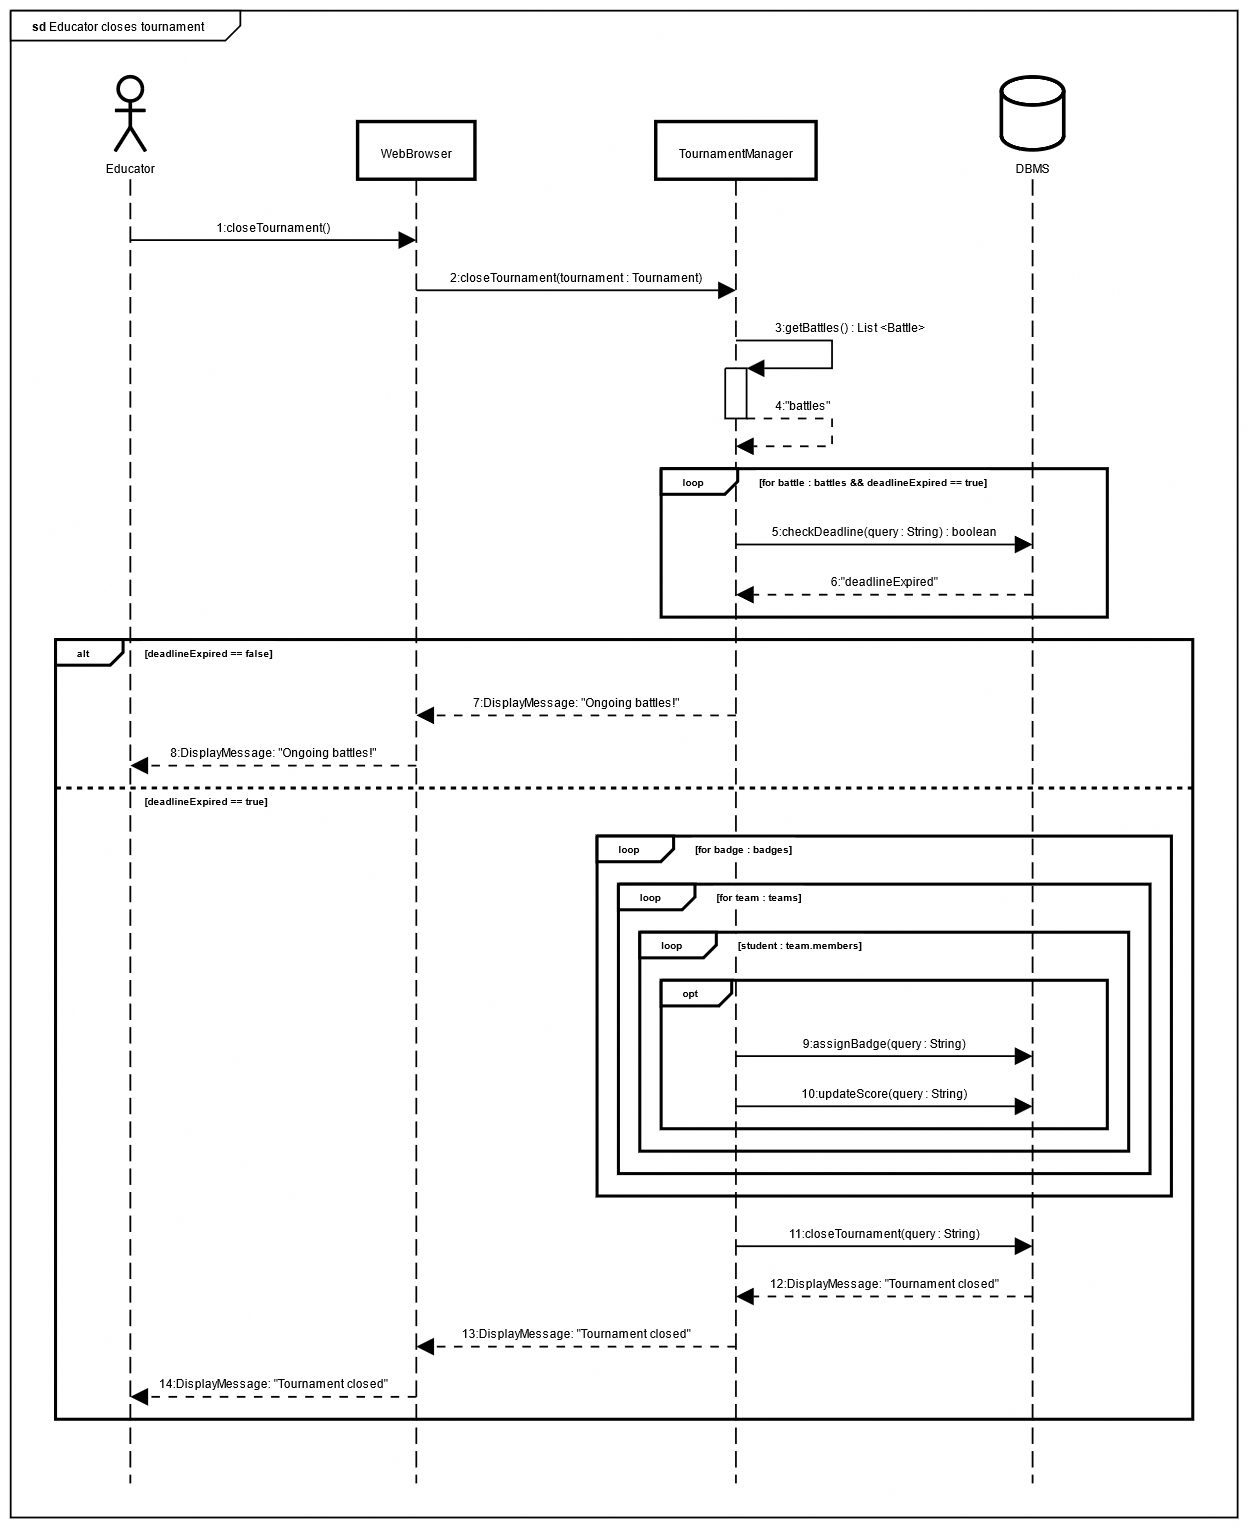
\includegraphics[width=1\linewidth]{Images/Sequence Diagrams/CloseTournament.png}
    \label{fig:enter-label}
\end{figure}

\clearpage

\subsection{Component Interfaces}
The following UML diagram displays how the CKB platform works, more specifically what methods are called, by which component and all the parameter and responses. The three main managers (UserManager, BattleManager and TournamentManager) are the main focus of the diagram, followed by the interaction with the EmailManager and the SecurityManager; all these managers, with their respective methods, are accessed by both Student Interface and Educator Interface accordingly. The Web Browser Manager was omitted for summary reasons, since it is only a intermediary between the users and the platform.

\begin{figure}[htbp]
    \centering
    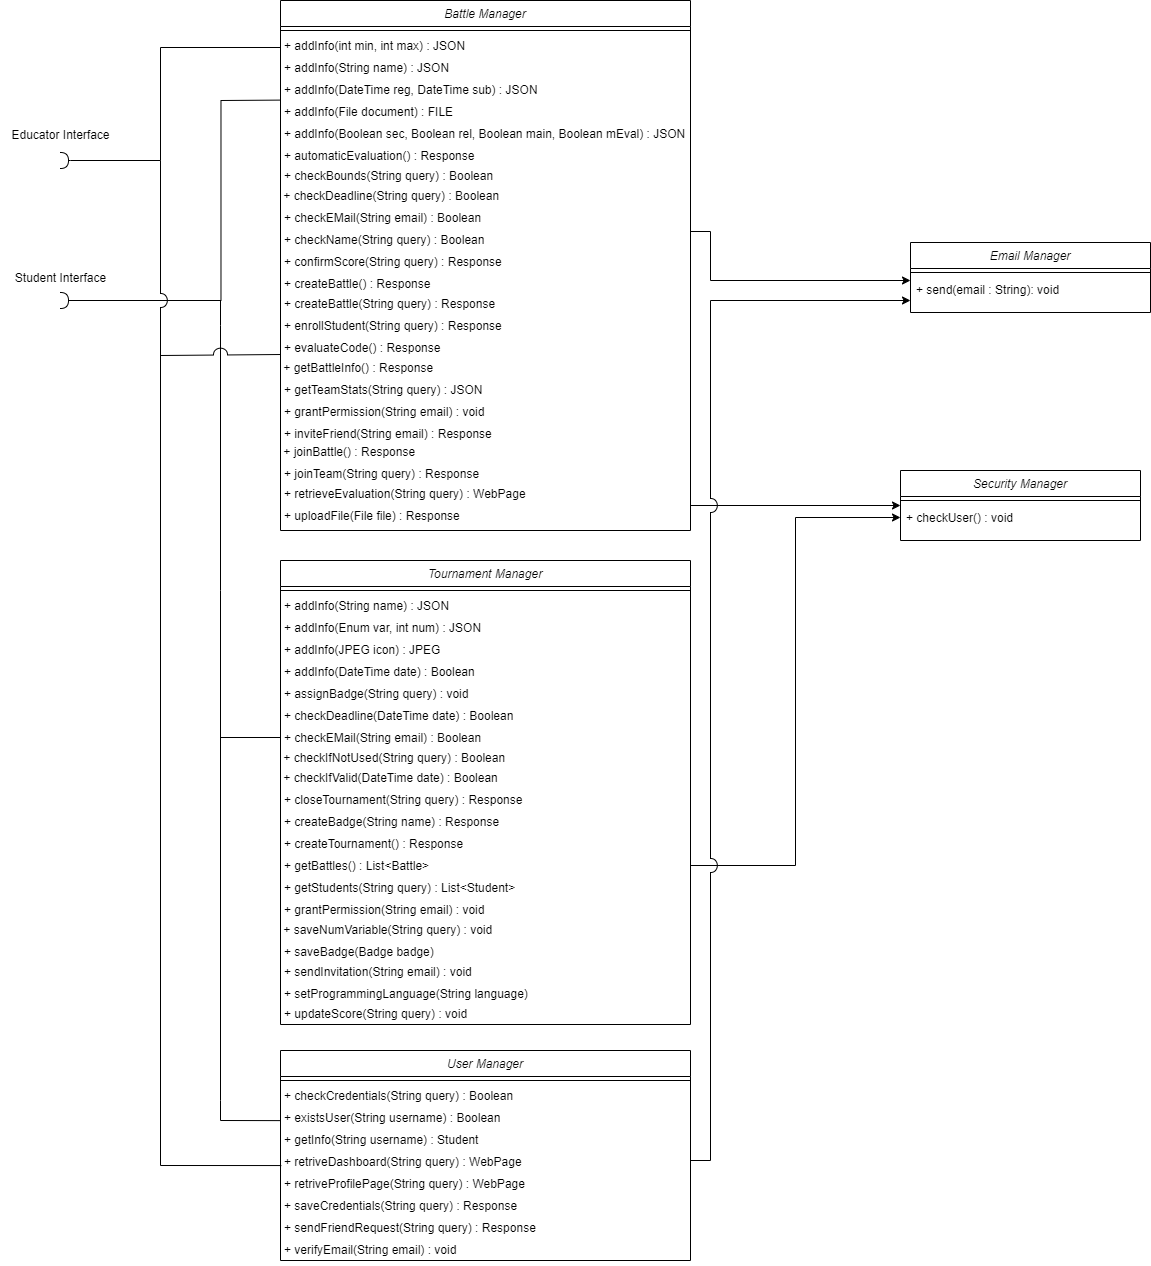
\includegraphics[scale=0.39]{Images/Diagrams/ComponentInterfaces.png}
\end{figure}

\clearpage

\begin{flushleft}
The following ER diagram in [Fig. 3], depicts the relations between the entities in the platform.
\end{flushleft}

\begin{figure}[htbp]
    \centering    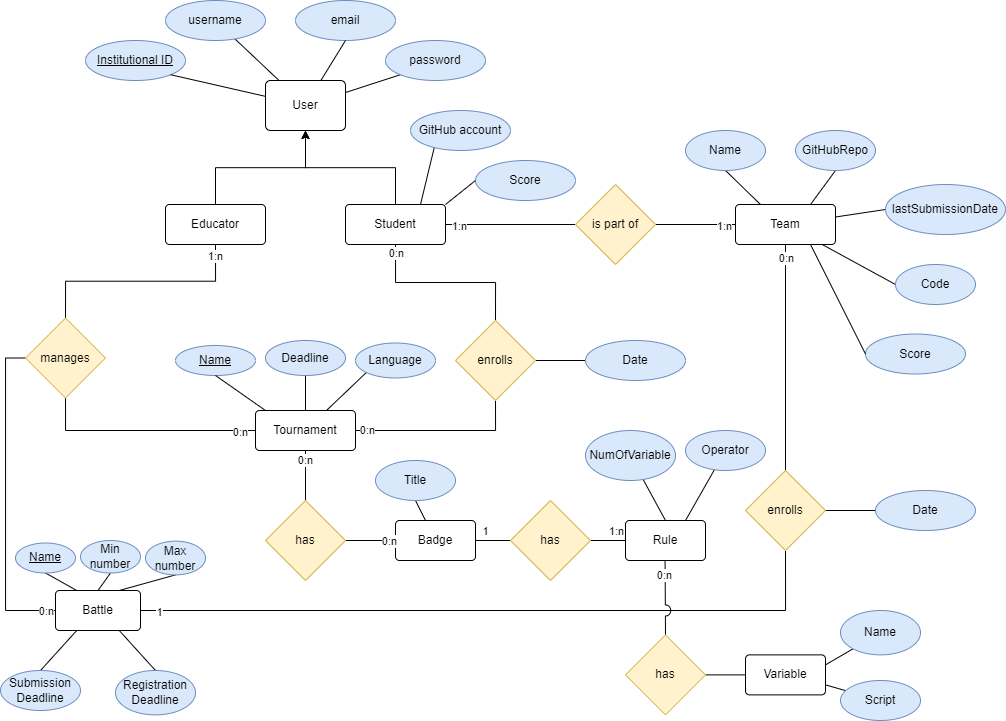
\includegraphics[width=1\linewidth]{Images/Diagrams/ERDiagram.png}
    \caption{ER Diagram}
    
\end{figure}

\subsection{Selected Architectural Styles and Patterns}

\subsubsection{RESTful Architecture}
The RESTful application will be utilized across the web-platform. This architecture adheres to the stateless principle, where the server lacks information about the client's state, which is managed directly on the client side. A notable feature of this architecture is the "code on demand," allowing the server to send code snippets to the client for local execution (typically within the web browser). This approach minimizes computational load on the server, fostering a dynamic service environment. The application is designed to leverage client-side scripting, meaning that all requests and page updates occur on the client side. This not only enhances user experience but also eliminates the need for page refreshing after each action.

\clearpage

\subsubsection{Four-tiered architecture}
We opted for this architecture for several compelling reasons:
\begin{itemize}
    \item \textbf{Flexibility:} Once the interfaces of S2B are defined, the internal logic becomes independent of external factors. This implies that each module can undergo improvements without necessitating changes to all others.
    
    \item \textbf{Scalability:} Dividing the application into multiple tiers ensures that the approach to scaling the architecture is applied only to the most critical components. This results in optimal performance while minimizing costs.
    
    \item \textbf{Load Distribution:} The inclusion of multiple application servers, facilitated by a load balancer, ensures a balanced distribution of requests. In contrast, relying on a single node could lead to overloading, risking system downtime.
\end{itemize}

\subsubsection{Model View controller (MVC)}
The Model-View-Controller (MVC) is a widely employed software design pattern for crafting user interfaces, strategically dividing the associated program logic into three interconnected elements. The primary objective is to segregate the internal representations of information from how information is both presented to and accepted from the user.
$\\$These three integral components are as follows:

\begin{itemize}
    \item \textbf{Model:} Positioned at the core of the pattern, the Model serves as the application's dynamic data structure, operating independently of the user interface. It directly oversees the management of data, logic, and application rules.
    
    \item \textbf{View:} Representations of information, such as charts, diagrams, or tables, fall under the purview of the View. Multiple views of the same information are possible, accommodating diverse needs, such as charts for the tournament statistics shown differently to students and educators.
    
    \item \textbf{Controller:} The Controller is responsible for accepting user input and translating it into commands for either the Model or the View, facilitating the interaction between the user and the application logic.
    
\end{itemize}

\clearpage

\subsection{Other Design Decisions}

\subsubsection{Thin client and Fat server}
The web application serves as the thin client in this architecture. The fundamental principle involves minimizing information stored on the client side, thereby confining the business logic exclusively to the server side. A stable connection between the components is imperative for the platform to function as intended. The primary advantage of adopting this implementation style is the minimal computational power required on the client machine.

\subsubsection{Scale-Out}
This approach involves replicating nodes anticipated to encounter bottlenecks, enhancing the overall scalability of the system. While this decision entails a greater deployment effort, it concurrently results in reduced hardware upgrade costs when system limits are approached. In essence, opting for a scale-out strategy is deemed preferable.
Upon segmentation, the system necessitates the inclusion of a load balancer to effectively reroute incoming requests to the node with the least workload, ensuring optimal distribution of tasks.

\subsubsection{Static Analysis Tools}
Static analysis tools play a crucial role in evaluating team code post-battle conclusion. We opted SonarQube to integrate within the Battle Manager since it evaluate the whole code with the specific criteria that the educator can select. Initially the platform clones the GitHub repository of the participating teams upon reaching the deadline. Subsequently the tool can start the evaluation process. It involves scrutinizing the code using parameters set by the educator at the time of battle creation. As outlined in the RASD, the evaluation criteria are Security, Reliability, and Maintainability. Once the process is finished the tool gives a total score on a 100 points obtainable by doing the average of the points scored between the criteria selected, the Functional Aspects and the timeliness. As said in the RASD the Functional Aspects are the test cased passed and the timeliness are the days passed from the registration to the last commit. The educator can confirm the score assigned by the tool or can opt to manually review the code and assign a score.


\subsubsection{Badge's rule language}
The CKB platform allows educators to create badges upon tournament creation. Badges are mainly composed by rules that must be satisfied to achieve them, but rules need variables to function. CKB gives partial access to the variables stored in the DBMS by the platform itself; by doing so, educators have the ability to use these variables to construct constraints and rules for a badge. Alternatively, if the educator wants to use specific custom variables, he/she needs to upload a script, locally written, so that CKB can reference to these variables flawlessly. To further simplify the badge creation process, CKB provides the educators with a straight forward language to build the rules; more specifically, the language only allows mathematical confrontations of variables and numbers, being integer, float or double. By doing so, many combinations and variations are still possible, while also granting limited access to DBMS and without making the process too complicated for the educators, since the whole tournament creation process, like all the other features embedded in the CKB platform, are meant to be easy to use for every user. As an example, if an educator wanted to make a badge that awards the student in a team who has the highest number of lines of code written, the educator should select the variables that store the lines written for every student and the variables concerning the teams and their participants. Once that is done, the educator implements some trivial mathematical confrontations between these numerical values and defines the rules for the badge to be awarded.

\clearpage



\section{User Interface Design}
This section is dedicated to illustrating the design of the primary screens within the User web portal, offering a detailed portrayal of the flow encompassing the main functionalities intended for the application. The flow is crafted in alignment with specific and illustrated input received from the end user. \textbf{It's essential to acknowledge} that, while most of the mockups from the RASD are incorporated and referenced, additional mockups have been generated and integrated into this section. The purpose is to enhance clarity and provide a more comprehensive understanding of the user experience by introducing a broader array of visual representations.



\subsection{Student Interface}
The student, at any given time, starting from his/her dashboard, can easily access a list of friends with a click of a button and, as shown in [Fig. 4], can search for a specific friend to see his/her profile or add a new friend by searching for a student's username.

\begin{figure}[htbp]
    \centering
    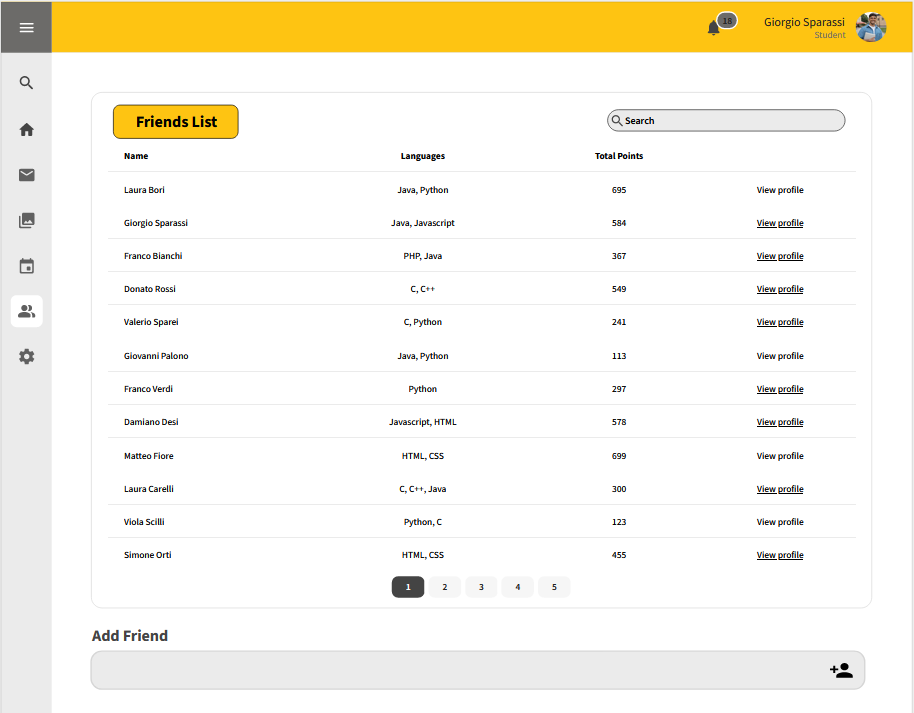
\includegraphics[width=1\linewidth]{Images/Interfaces/FriendsRequest.PNG}
    \caption{Student sends a friend request}
    \label{fig:enter-label}
\end{figure}

\pagebreak

\begin{flushleft}  
Any user, both educators and students, at any given time, starting from his/her dashboard, can easily look for a student's profile, as shown in [Fig. 5]. For simplicity, and since it would probably be the most common scenario, we are showing this interface from the Student's perspective. By searching the username of another student and clicking the button, the student is redirected onto the student's profile page. Here he/she is presented with a variety of information, such as the number of badges awarded, the tournaments the student is enrolled in, the number of friends in common and much more.
\end{flushleft}
\begin{figure}[htbp]
    \centering
    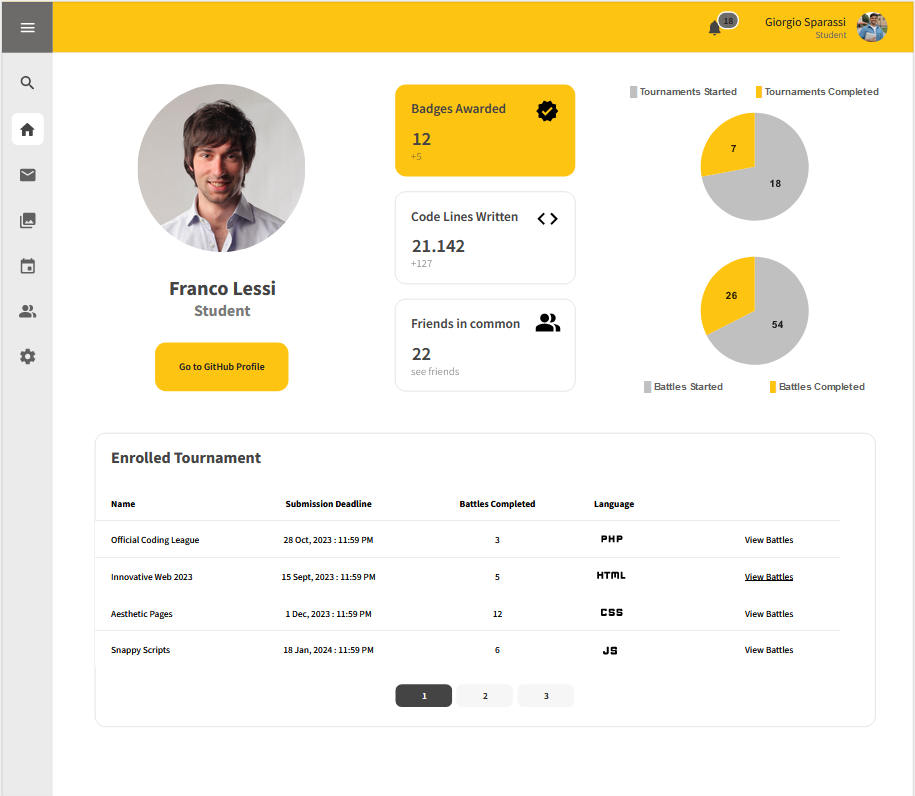
\includegraphics[width=1\linewidth]{Images/Interfaces/StudentProfile.PNG}
    \caption{Student sends a friend request}
    \label{fig:enter-label}
\end{figure}

\pagebreak

\begin{flushleft}
When adding or creating a badge, the educator might want to create new rules. This mock up in [Fig. 6] shows how he/she can create a rule using some variables already provided by the CKB platform, a mathematical operator and a number of his/her choice. Alternatively, the educator can decide to create a new variable by uploading a script, which must have been created locally, and by giving it a name. Once the variable is added and saved, it can be used indefinitely in the future for other rules and/or other badges.
\end{flushleft}
\begin{figure}[htbp]
    \centering
    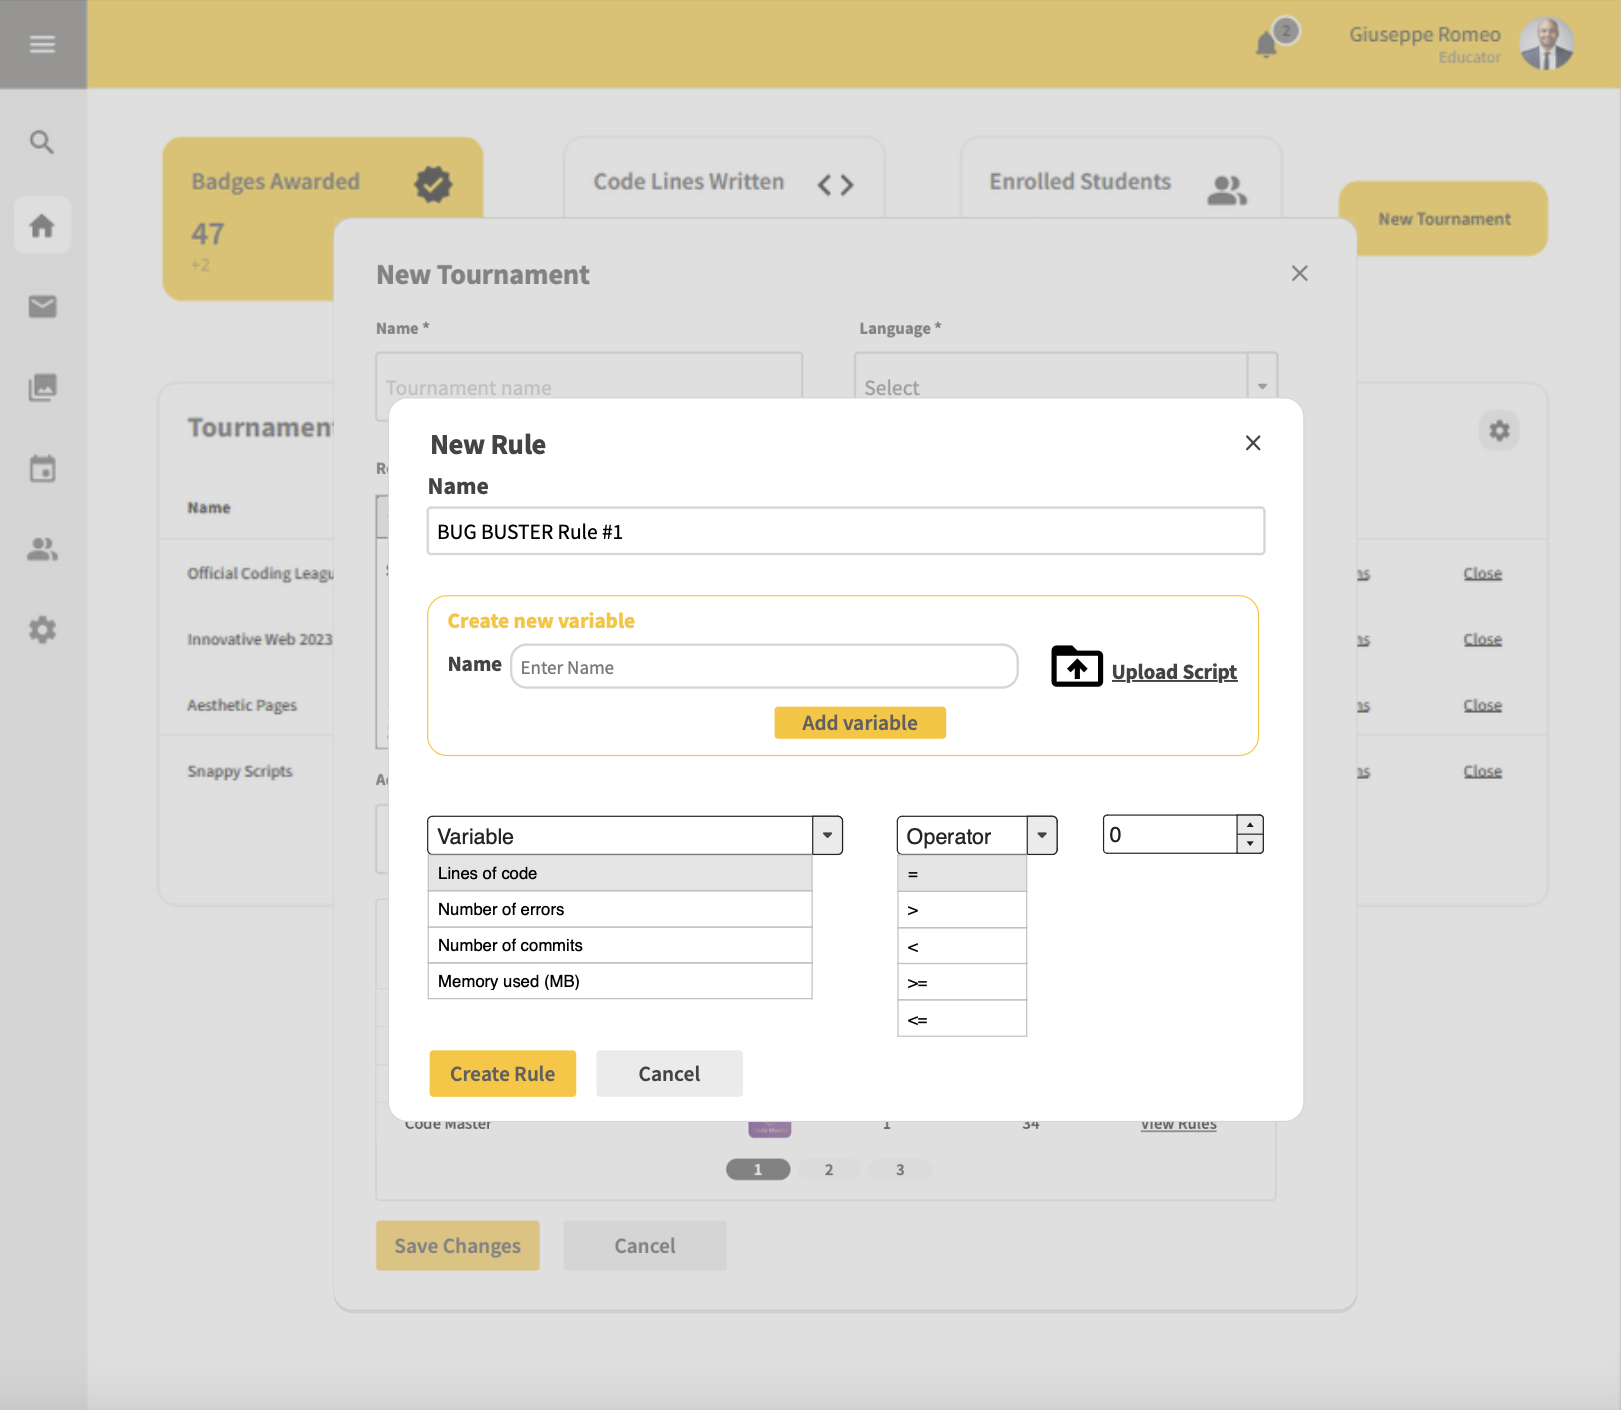
\includegraphics[width=1\linewidth]{Images/Interfaces/CreateRule.PNG}
    \caption{Educator creates rule}
    \label{fig:enter-label}
\end{figure}
\clearpage

\section{Requirements Traceability}

\begin{table}[htbp]
\begin{tabular}{|l|p{12cm}|}
    \hline
    \textbf{Requirement:} & [R1] The system allows a registered student to accept a tournament invitation\\
    \hline
    \textbf{Components:} & \begin{itemize}
        \item \textbf{TournamentManager} in order to accept the invitation received and be enrolled in the tournament.
        \item \textbf{EmailManager} in order to receive the invitation.
    \end{itemize}\\
    \hline
\end{tabular}
\end{table}


\begin{table}[htbp]
\begin{tabular}{|l|p{12cm}|}
    \hline
    \textbf{Requirement:} & [R2] The system allows a registered student to select a battle to join\\
    \hline
    \textbf{Components:} & \begin{itemize}
        \item \textbf{BattleManager} in order to be able to retrieve the battles and to register to a battle.
    \end{itemize}\\
    \hline
\end{tabular}
\end{table}

\begin{table}[htbp]
\begin{tabular}{|l|p{12cm}|}
    \hline
    \textbf{Requirement:} & [R3] The system allows a registered student retrieve a battles’ list for each tournament\\
    \hline
    \textbf{Components:} & \begin{itemize}
        \item \textbf{TournamentManager} to allow the student to consult tournament's info, including the battles' list.
    \end{itemize}\\
    \hline
\end{tabular}
\end{table}

\begin{table}[htbp]
\begin{tabular}{|l|p{12cm}|}
    \hline
    \textbf{Requirement:} & [R4] The system allows a registered user to retrieve a list of students\\
    \hline
    \textbf{Components:} & \begin{itemize}
        \item \textbf{UserManager} to allow users to search for a student's username on the platform.
    \end{itemize}\\
    \hline
\end{tabular}
\end{table}

\begin{table}[htbp]
\begin{tabular}{|l|p{12cm}|}
    \hline
    \textbf{Requirement:} & [R5] The system allows a registered student to invite a student in his/her team\\
    \hline
    \textbf{Components:} & \begin{itemize}
        \item \textbf{UserManager} to retrieve the student's email and other useful data, such as friendship status, which could come in handy when inviting to join a team.
        \item \textbf{EmailManager} to allow the system to send an invitation via email.
        \item \textbf{BattleManager} to manage the team, verify size boundaries and deadlines of the battle.
    \end{itemize}\\
    \hline
\end{tabular}
\end{table}

\begin{table}[htbp]
\begin{tabular}{|l|p{12cm}|}
    \hline
    \textbf{Requirement:} & [R6] The system allows a registered student to create a team\\
    \hline
    \textbf{Components:} & \begin{itemize}
        \item \textbf{BattleManager} to allow team creation for a specific battle.
    \end{itemize}\\
    \hline
\end{tabular}
\end{table}

\begin{table}[htbp]
\begin{tabular}{|l|p{12cm}|}
    \hline
    \textbf{Requirement:} & [R7] The system generates a tournament invitation link for all students\\
    \hline
    \textbf{Components:} & \begin{itemize}
        \item \textbf{EmailManager} to send invitation links via email.
        \item \textbf{UserManager} to retrieve students' email addresses.
        \item \textbf{TournamentManager} to access the tournament info, check deadline and create a valid enrolment link.
    \end{itemize}\\
    \hline
\end{tabular}
\end{table}

\begin{table}[htbp]
\begin{tabular}{|l|p{12cm}|}
    \hline
    \textbf{Requirement:} & [R8] The system allows a registered educator to set up the tournament parameters\\
    \hline
    \textbf{Components:} & \begin{itemize}
        \item \textbf{TournamentManager} to create the tournament and allow the tweaking of its parameters.
    \end{itemize}\\
    \hline
\end{tabular}
\end{table}

\begin{table}[htbp]
\begin{tabular}{|l|p{12cm}|}
    \hline
    \textbf{Requirement:} & [R9] The system allows a registered educator to grant access to other educators\\
    \hline 
    \textbf{Components:} & \begin{itemize}
        \item \textbf{TournamentManager} to change permissions' allowance inside the tournament.
        \item \textbf{UserManager} to retrieve educators' email addresses.
        \item \textbf{EmailManager} to send the notification email to educators.
    \end{itemize}\\
    \hline
\end{tabular}
\end{table}

\begin{table}[htbp]
\begin{tabular}{|l|p{12cm}|}
    \hline
    \textbf{Requirement:} & [R10] The system allows a registered educator to create badges\\
    \hline
    \textbf{Components:} & \begin{itemize}
        \item \textbf{TournamentManager} to establish variables and rules for a badge and, eventually, to assign them.
    \end{itemize}\\
    \hline
\end{tabular}
\end{table}

\begin{table}[htbp]
\begin{tabular}{|l|p{12cm}|}
    \hline
    \textbf{Requirement:} & [R11] The system allows a registered educator to set up the battle parameters\\
    \hline
    \textbf{Components:} & \begin{itemize}
        \item \textbf{BattleManager} to create the battle and allow the tweaking of its parameters.
    \end{itemize}\\
    \hline
\end{tabular}
\end{table}

\begin{table}[htbp]
\begin{tabular}{|l|p{12cm}|}
    \hline
    \textbf{Requirement:} & [R12] The system displays the automated evaluation score, calculated for the team’s project\\
    \hline
    \textbf{Components:} & \begin{itemize}
        \item \textbf{BattleManager} to allow educators to access the evaluation page of the battle and to access the score, automatically computed by the platform, for each team.
    \end{itemize}\\
    \hline
\end{tabular}
\end{table}

\begin{table}[htbp]
\begin{tabular}{|l|p{12cm}|}
    \hline
    \textbf{Requirement:} & [R13] The system allows a registered user to see a student’s public profile\\
    \hline
    \textbf{Components:} & \begin{itemize}
        \item \textbf{EducatorManager} to allow an educator to search for a student.
        \item \textbf{StudentManager} to allow a student to search for another student.
    \end{itemize}\\
    \hline
\end{tabular}
\end{table}

\clearpage

\begin{flushleft}
Furthermore, the S2B's attributes and qualities are guaranteed by the following design choices:
\end{flushleft}

\begin{itemize}
    \item \textbf{Ease of use} - User friendly design is ensured through an interface characterized by simplicity, minimalism, and intuitiveness. Given that the primary focus of the platform is to teach in an entertaining and easy way, the user experience is intentionally crafted to be straightforward. The interface features only a handful of buttons, each with clear and precise functionalities. The overarching goal is to facilitate the use of the platform for its most important functions. This streamlined design approach aims to enhance user satisfaction and efficiency, prioritizing a seamless experience for users interacting with the platform.
    \item \textbf{Security} - Security measures are upheld by implementing encrypted communication between the client and server. When the client accesses the system via the web interface, the connection operates through the HTTPS protocol, ensuring a secure and encrypted data exchange.
    \item \textbf{Modularity and Maintainability} - Maintainability is achieved through the strategic implementation of modularity. The platform is structured by dividing it into smaller, self-contained units known as modules. These modules work in tandem, interacting with each other to deliver the desired service. This modular approach simplifies the maintenance process by isolating specific functionalities into manageable components. It facilitates updates, debugging, and enhancements without disrupting the entire system, promoting a more efficient and sustainable development and maintenance environment.
\end{itemize}

\pagebreak


\section{Implementation, Integration and Test Plan}
This section delves into the implementation of the system, outlining the integration of its components and detailing the methods for validation and verification. It is crucial to acknowledge that it is not possible to show the total absence of bugs. Therefore, the testing procedures adopted for the system aim to unearth the majority of application bugs prior to each release. The integration and implementation are strongly related, often resulting in the integration order coinciding with the implementation sequence. Thus, while the initial section is dedicated to the implementation strategy, due consideration is given to the integration test plan during its formulation. Emphasizing the importance of comprehensive documentation, it is crucial that the written code is well-commented and documented, potentially utilizing tools like Javadoc. This practice ensures clarity and understanding, facilitating not only the implementation process but also aiding in ongoing maintenance and potential future developments.

\subsection{Implementation}
CKB will be implemented with a combinations of thread strategy and top-down strategy to exploit the pros of these approaches. Indeed, using the top-down strategy allows us to start building functionalities and test them with stubs as they are developed, while always replacing outdated and used stubs; at the same time, following the thread strategy gives us the ability to provide user-visible features more quickly, thus making the development progress much more clear and visible to end users and stakeholders, also helping in the testing phase, explained later on in this document. The feature to implement in the system are derived from the system requirements listed in the RASD, but is worth noting that some require the implementation of entire components to be satisfied, while others just need the implementation of smaller portions of one or more of them.

\clearpage

\subsection{Integration}
In this section we indicate what modules and/or components are integrated for each development stage.
$\\$The followinig figure [Fig. 7] elucidates that the initial step involves building the Database Management System (DBMS), succeeded by the subsequent development of key application components that leverage its functionalities.

\begin{figure}[htbp]
    \centering
    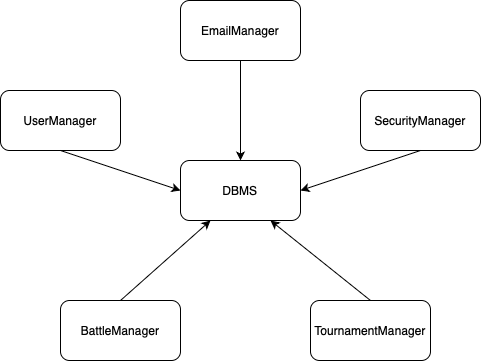
\includegraphics[scale=0.55]{Images/Diagrams/ComponentsIntegration.png}
    \caption{Components Diagram}
    \label{fig:enter-label}
\end{figure}

\begin{flushleft}
    After that, the integration of the User Manager takes place. This component facilitates both educators and students in harnessing the full range of functionalities provided by the platform, as illustrated in [Fig. 8].
\end{flushleft}

\begin{figure}[htbp]
    \centering
    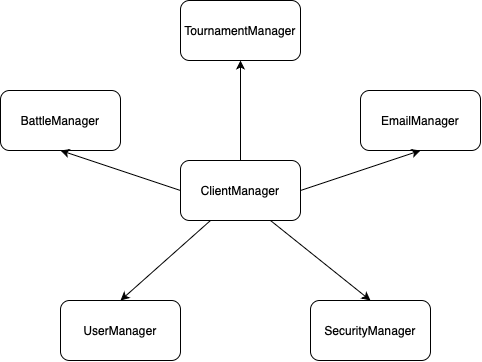
\includegraphics[scale=0.55]{Images/Diagrams/ClientManager.png}
    \caption{Client Manager Diagram}
    \label{fig:enter-label}
\end{figure}

\clearpage

\begin{flushleft}
    Ultimately, the integration of the web server module and the Web Browser becomes feasible. This crucial step is essential to enable effective client-server communication. Figure 9 visually represents this final phase. Additionally, in tandem with this integration, as depicted in [Fig. 10], the client will be connected to the GitHub API.
\end{flushleft}

\begin{figure}[htbp]
    \centering
    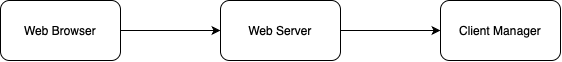
\includegraphics[scale=0.55]{Images/Diagrams/WebServer.png}
    \caption{Web Integration}
    \label{fig:enter-label}
\end{figure}

\begin{figure}[htbp]
    \centering
    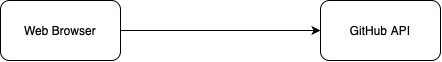
\includegraphics[scale=0.55]{Images/Diagrams/GitHub.png}
    \caption{GitHub API}
    \label{fig:enter-label}
\end{figure}

\subsection{Test Plan}
The CKB platform must be submitted to various test batteries, all having different scopes and different levels of test granularity. It is crucial that, during every stage of development, all the components and modules so far developed are tested individually, to ensure their correct behavior, evaluate their performance and if they satisfy the expectations set for that development stage. Doing so not only minimizes the chance of having a finished product that does not meet performance expectations, but also makes fixing bugs much easier, given that spotting them early on also increases the chance of fixing them in a more efficient and quick way. It may be needed, given that some components may not work in isolation, to realize specific temporary modules that simulate the behavior of the surrounding (and possibly missing) ones. At this stage of development is very useful to receive some feedback, both from stakeholder and end users, whenever a new feature has been implemented or an existing feature has been heavily modified and updated. To enhance and make this process much easier for the users, the development team could provide some brief documentation, stating all the new features implemented and what they offer. In this way, stakeholders and users can raise any concern if some of their needs are not met and check precisely whether the features implemented work as they intended. 
Once the system has been implemented and integrated, with all the relative testing phases, it must be tested entirely to verify that all the features requested have been fully and correctly developed and that the system complies with the requirements, both functional and non, stated in the RASD.
The development team might as well decide to release some alpha version of the finished product only to some users and, later on, to distribute a beta version, where the major bugs found in the alpha version are fixed, to the stakeholders. This approach grants a more successful product launch, having satisfies the requested needs of the stakeholders and having fixed the major and minor, but not all, bugs. The main steps of this testing, defined as system testing, are the following:

\clearpage

\begin{itemize}
    \item \textbf{Performance}: to spot inefficiencies in the system's functionalities that may lead to bottlenecks or other problems affecting the performances. To proceed with this test phase, a performance target and some test workloads, resembling the real effective load that the system will handle once deployed, are needed. It may be useful to include some stress testing in this phase, to understand how well the system recovers itself after heavy usage and potential failure.
    \item \textbf{Functionalities}: to ensure that the system satisfies all the requirements specified in the RASD and, potentially, to plan the introduction of new features that might enhance the user experience.
    \item \textbf{Usability}: since the platform will be used by any kind of user, both experienced and not, it is crucial to ensure the swiftness of the user experience when performing the main tasks. This phase might also hint the designers with some improvements with the UI and the UX to further enhance the experience for the user.
\end{itemize}

\clearpage

\section{Effort Spent}

\begin{table}[H]
    \centering
    \begin{tabular}{|c|c|c|c|c|c|}
    \hline
    \textbf{Student} & \textbf{Section 1} & \textbf{Section 2} & \textbf{Section 3} & \textbf{Section 4}  & \textbf{Section 5}\\
    \hline
    Filippo Gentili & 2 & 10 & 3 & 1 & 1\\
    \hline
    Emanuele Greco & 2 & 9 & 3 & 1 & 3\\
    \hline
    Marco Giulio Grilli & 2 & 10 & 2 & 1 & 2\\
    \hline
    \end{tabular}
\end{table}

\section{References}
In this Design Document we have used the following references:

$\\$Websites that have a similar use case:
\begin{itemize}
    \item \href{https://www.leetcode.com}{LeetCode}
    \item \href{https://www.hackerrank.com}{HackerRank}
    \item \href{https://www.codewars.com}{CodeWars}
    \item \href{https://www.github.com}{GitHub}
\end{itemize}

$\\$Websites used for the moqups:
\begin{itemize}
    \item \href{https://www.moqups.com}{Moqups}
    \item \href{https://www.designs.ai}{Designs}
    \item \href{https://www.looka.com}{Looka}
\end{itemize}

$\\$Websites used for the diagrams:
\begin{itemize}
    \item \href{https://www.draw.io}{Draw}
    \item \href{https://sequencediagram.org}{SequenceDiagram}
\end{itemize}

$\\$Website used for the static analysis tools
\begin{itemize}
    \item \href{https://www.sonarsource.com/products/sonarqube/} {SonarQube}
\end{itemize}

\end{document}
